% Copyright (C) Tanner Koza - All Rights Reserved
% Unauthorized copying of this file, via any medium is strictly prohibited
% Written by Tanner Koza <jtk0018@auburn.edu>, October 2022

% PROBLEM 3
\question
Consider the time-varying coordinate transformation matrix $C^{n}_{b}$ given below that describes the orientation of the body frame as it rotates with respect to the navigation frame.

\[C^n_b =
    \begin{bmatrix}
        cos(t)  & sin(t)sin(t^2)  & sin(t)cos(t^2) \\
        0       & cos(t^2)        & -sin(t^2)      \\
        -sin(t) & cos(t) sin(t^2) & cos(t)cos(t^2) \\
    \end{bmatrix} \]

\begin{parts}

    \part{Compute expressions for $\psi$,$\theta$, and $\phi$ based on the fixed-axis definition of roll, pitch, yaw assuming a 1,2,3 series of rotations (roll, pitch, yaw).}

    \solution
    Euler angles from a 1-2-3 rotation can be extracted using the following:

    \begin{equation*}
        \begin{split}
            \phi & = tan^{-1}\left(\frac{-C_{23}}{C_{33}}\right) \\
            \theta & = sin^{-1}(-C_{13})\\
            \psi & = tan^{-1}\left(\frac{-C_{12}}{C_{11}}\right)\\
        \end{split}
    \end{equation*}

    \part{Use MATLAB to plot $\psi$, $\theta$, and $\phi$ as a function of time.}

    A simulation of the rotations was conducted for 10 seconds at 100 Hz. Figure~\ref*{fig:euler} depicts the resulting Euler angles.

    \begin{figure}[!ht]
        \centering
        % Copyright (C) Tanner Koza - All Rights Reserved
% Unauthorized copying of this file, via any medium is strictly prohibited
% Written by Tanner Koza <jtk0018@auburn.edu>, October 2022

% This file was created by matlab2tikz.
%
\definecolor{mycolor1}{rgb}{0.00000,0.44700,0.74100}%
\definecolor{mycolor2}{rgb}{0.85000,0.32500,0.09800}%
\definecolor{mycolor3}{rgb}{0.92900,0.69400,0.12500}%
%
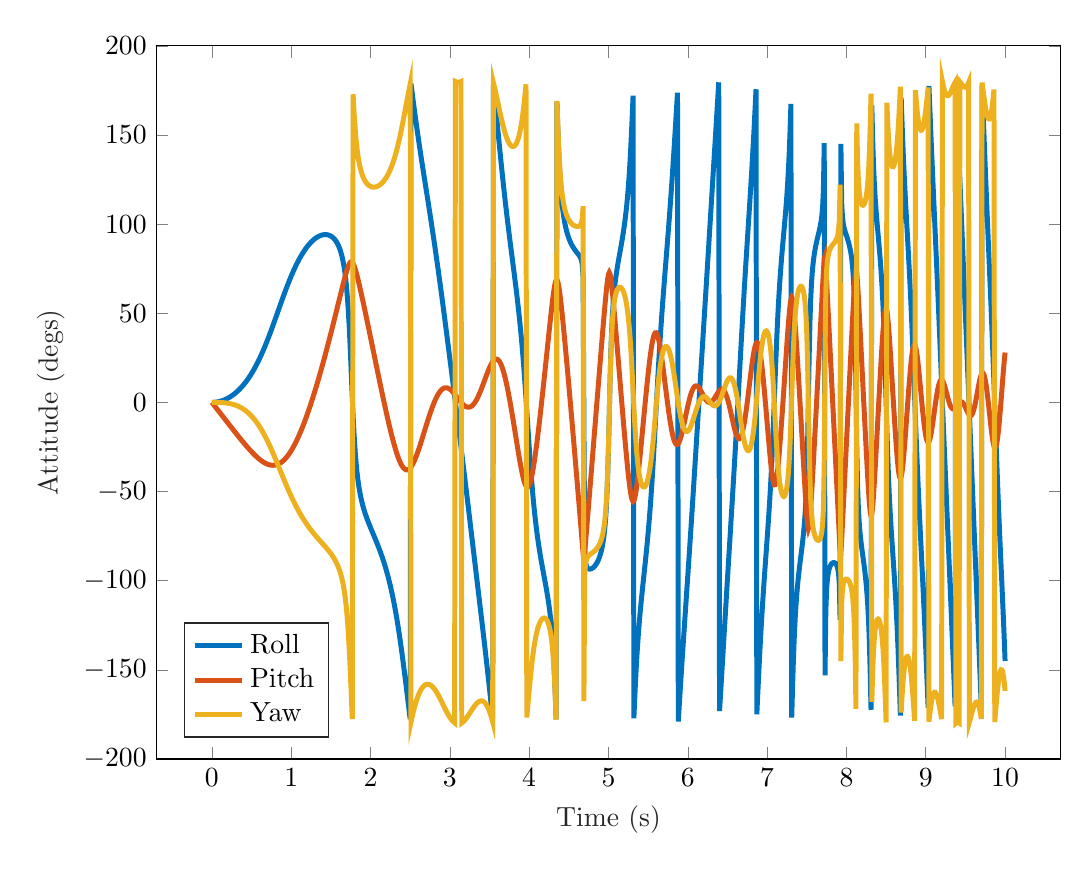
\begin{tikzpicture}

\begin{axis}[%
width=4.521in,
height=3.566in,
at={(0.758in,0.481in)},
scale only axis,
xmin=-0.7,
xmax=10.7,
xlabel style={font=\color{white!15!black}},
xlabel={Time (s)},
ymin=-200,
ymax=200,
ylabel style={font=\color{white!15!black}},
ylabel={Attitude (degs)},
axis background/.style={fill=white},
legend style={at={(0.03,0.03)}, anchor=south west, legend cell align=left, align=left, draw=white!15!black}
]
\addplot [color=mycolor1, line width=1.8pt]
  table[row sep=crcr]{%
0	0\\
0.01	0.00572986444214099\\
0.02	0.0229228962311728\\
0.03	0.0515894150449157\\
0.04	0.0917466346175419\\
0.05	0.143418684044976\\
0.06	0.2066366374085\\
0.07	0.281438551509496\\
0.08	0.367869511444574\\
0.09	0.465981683683286\\
0.1	0.575834376239283\\
0.11	0.697494105449392\\
0.12	0.831034668792693\\
0.13	0.976537223092432\\
0.14	1.13409036734643\\
0.15	1.3037902293256\\
0.16	1.48574055496418\\
0.17	1.68005279943808\\
0.18	1.88684621868835\\
0.19	2.10624795999378\\
0.2	2.33839315002879\\
0.21	2.58342497865891\\
0.22	2.84149477652462\\
0.23	3.11276208424409\\
0.24	3.39739471082499\\
0.25	3.69556877861327\\
0.26	4.00746875182259\\
0.27	4.33328744537902\\
0.28	4.67322601048269\\
0.29	5.02749389292923\\
0.3	5.39630875984895\\
0.31	5.77989639011174\\
0.32	6.17849052320958\\
0.33	6.59233266096943\\
0.34	7.02167181596766\\
0.35	7.46676420001713\\
0.36	7.92787284558373\\
0.37	8.40526715246586\\
0.38	8.89922235154657\\
0.39	9.41001887691214\\
0.4	9.93794163713568\\
0.41	10.4832791760635\\
0.42	11.0463227130333\\
0.43	11.6273650521186\\
0.44	12.2266993497529\\
0.45	12.8446177299765\\
0.46	13.4814097365913\\
0.47	14.137360611747\\
0.48	14.8127493909556\\
0.49	15.5078468052809\\
0.5	16.2229129825268\\
0.51	16.9581949407029\\
0.52	17.7139238689282\\
0.53	18.490312193292\\
0.54	19.287550428084\\
0.55	20.1058038162658\\
0.56	20.945208767124\\
0.57	21.8058691037448\\
0.58	22.6878521382839\\
0.59	23.5911845989611\\
0.6	24.5158484392364\\
0.61	25.4617765666598\\
0.62	26.4288485362978\\
0.63	27.416886261291\\
0.64	28.4256498007671\\
0.65	29.4548332927891\\
0.66	30.5040611069521\\
0.67	31.5728842973309\\
0.68	32.6607774413416\\
0.69	33.7671359533365\\
0.7	34.8912739629992\\
0.71	36.0324228474753\\
0.72	37.1897305023287\\
0.73	38.3622614295807\\
0.74	39.5489977111167\\
0.75	40.7488409225728\\
0.76	41.9606150265614\\
0.77	43.1830702650203\\
0.78	44.4148880490233\\
0.79	45.6546868211789\\
0.8	46.9010288415309\\
0.81	48.152427823552\\
0.82	49.4073573233471\\
0.83	50.6642597635651\\
0.84	51.9215559547035\\
0.85	53.1776549613754\\
0.86	54.4309641503883\\
0.87	55.6798992517066\\
0.88	56.9228942627999\\
0.89	58.1584110315553\\
0.9	59.3849483626134\\
0.91	60.6010505062042\\
0.92	61.8053149066233\\
0.93	62.9963991085473\\
0.94	64.173026742501\\
0.95	65.3339925349542\\
0.96	66.4781663127626\\
0.97	67.6044959950773\\
0.98	68.7120095876311\\
0.99	69.7998162138189\\
1	70.8671062337568\\
1.01	71.9131505162099\\
1.02	72.9372989387971\\
1.03	73.9389781992103\\
1.04	74.9176890244832\\
1.05	75.8730028668435\\
1.06	76.8045581737116\\
1.07	77.7120563163282\\
1.08	78.5952572566984\\
1.09	79.453975026415\\
1.1	80.2880730838405\\
1.11	81.0974596084207\\
1.12	81.8820827828782\\
1.13	82.6419261059323\\
1.14	83.3770037702273\\
1.15	84.0873561324671\\
1.16	84.7730452954745\\
1.17	85.4341508150787\\
1.18	86.0707655384225\\
1.19	86.6829915744728\\
1.2	87.2709363921896\\
1.21	87.8347090369134\\
1.22	88.3744164510037\\
1.23	88.8901598805192\\
1.24	89.3820313456807\\
1.25	89.8501101488929\\
1.26	90.2944593900978\\
1.27	90.7151224550624\\
1.28	91.1121194377114\\
1.29	91.4854434526358\\
1.3	91.8350567882472\\
1.31	92.1608868444765\\
1.32	92.4628217911747\\
1.33	92.740705874141\\
1.34	92.9943342845962\\
1.35	93.2234474944622\\
1.36	93.4277249434236\\
1.37	93.6067779436949\\
1.38	93.7601416437784\\
1.39	93.887265862108\\
1.4	93.9875045638287\\
1.41	94.0601037071488\\
1.42	94.1041871272265\\
1.43	94.1187400521902\\
1.44	94.1025897533983\\
1.45	94.0543827148502\\
1.46	93.9725575573844\\
1.47	93.8553127620904\\
1.48	93.7005679910293\\
1.49	93.5059174840969\\
1.5	93.2685735945007\\
1.51	92.9852979788514\\
1.52	92.6523172359562\\
1.53	92.2652188284304\\
1.54	91.8188218363593\\
1.55	91.3070153614918\\
1.56	90.7225550551145\\
1.57	90.0568050476858\\
1.58	89.2994081874405\\
1.59	88.4378615020626\\
1.6	87.4569655862973\\
1.61	86.3381054337114\\
1.62	85.0583052177014\\
1.63	83.5889799904732\\
1.64	81.8942834534236\\
1.65	79.9289261010245\\
1.66	77.6353235007644\\
1.67	74.9399617957112\\
1.68	71.7490157331228\\
1.69	67.9437068741341\\
1.7	63.3770328728327\\
1.71	57.8760196090676\\
1.72	51.2582881052274\\
1.73	43.3774802022443\\
1.74	34.2107511896169\\
1.75	23.9725602468031\\
1.76	13.1734408057345\\
1.77	2.51527562140039\\
1.78	-7.35678119551618\\
1.79	-16.0572969786717\\
1.8	-23.4864164762886\\
1.81	-29.7332877495789\\
1.82	-34.9679175077942\\
1.83	-39.3723478880052\\
1.84	-43.1096039532197\\
1.85	-46.3147062247692\\
1.86	-49.0955316106208\\
1.87	-51.5369905201129\\
1.88	-53.7056694036476\\
1.89	-55.653917696586\\
1.9	-57.42314071845\\
1.91	-59.0463497687691\\
1.92	-60.5501026372001\\
1.93	-61.9559711639888\\
1.94	-63.2816512600879\\
1.95	-64.5418056444079\\
1.96	-65.74870741816\\
1.97	-66.9127350456889\\
1.98	-68.0427560386453\\
1.99	-69.1464268281843\\
2	-70.2304291299157\\
2.01	-71.3006578698485\\
2.02	-72.3623719174282\\
2.03	-73.4203160726442\\
2.04	-74.4788206940564\\
2.05	-75.5418838291386\\
2.06	-76.6132395709562\\
2.07	-77.6964155106087\\
2.08	-78.7947815071818\\
2.09	-79.9115915011583\\
2.1	-81.0500197131614\\
2.11	-82.2131922679065\\
2.12	-83.4042150412311\\
2.13	-84.6261983292872\\
2.14	-85.8822787704892\\
2.15	-87.1756388024041\\
2.16	-88.5095237991559\\
2.17	-89.8872569032114\\
2.18	-91.3122514327785\\
2.19	-92.7880206074762\\
2.2	-94.3181841862938\\
2.21	-95.9064714499708\\
2.22	-97.5567197830225\\
2.23	-99.2728679189005\\
2.24	-101.058942708363\\
2.25	-102.919038063368\\
2.26	-104.857284530014\\
2.27	-106.87780777537\\
2.28	-108.984674165949\\
2.29	-111.181821613653\\
2.3	-113.472974025578\\
2.31	-115.861538087389\\
2.32	-118.350481815843\\
2.33	-120.942195414522\\
2.34	-123.638336522697\\
2.35	-126.439663985439\\
2.36	-129.345866746895\\
2.37	-132.3553972236\\
2.38	-135.465321258038\\
2.39	-138.671199041987\\
2.4	-141.967012669025\\
2.41	-145.345155617813\\
2.42	-148.796496969635\\
2.43	-152.310528285629\\
2.44	-155.875594014959\\
2.45	-159.479197816449\\
2.46	-163.108368484132\\
2.47	-166.750061773519\\
2.48	-170.391569748759\\
2.49	-174.020908263443\\
2.5	-177.627156059304\\
2.51	178.799274878256\\
2.52	175.266449855649\\
2.53	171.780806282133\\
2.54	168.347128234794\\
2.55	164.968590215456\\
2.56	161.646855837523\\
2.57	158.382215789903\\
2.58	155.173749947315\\
2.59	152.019500351378\\
2.6	148.9166443739\\
2.61	145.861660180845\\
2.62	142.850479272573\\
2.63	139.878623160635\\
2.64	136.941323055943\\
2.65	134.033622779521\\
2.66	131.150466012589\\
2.67	128.286769551069\\
2.68	125.437484501131\\
2.69	122.597647421432\\
2.7	119.762423346961\\
2.71	116.927142467626\\
2.72	114.087332017627\\
2.73	111.238744683774\\
2.74	108.377384578088\\
2.75	105.499531551726\\
2.76	102.601764359202\\
2.77	99.6809829174055\\
2.78	96.7344296462001\\
2.79	93.7597096303088\\
2.8	90.7548091114029\\
2.81	87.7181116128825\\
2.82	84.6484108281817\\
2.83	81.5449192791314\\
2.84	78.4072716876018\\
2.85	75.2355220146244\\
2.86	72.0301332174184\\
2.87	68.7919589625217\\
2.88	65.5222168120748\\
2.89	62.2224527610554\\
2.9	58.8944974272778\\
2.91	55.5404146554275\\
2.92	52.1624437562773\\
2.93	48.7629370236076\\
2.94	45.3442945158858\\
2.95	41.9088983245377\\
2.96	38.4590486527407\\
2.97	34.9969039881975\\
2.98	31.5244274750355\\
2.99	28.0433412920892\\
3	24.555090456552\\
3.01	21.0608170289861\\
3.02	17.5613452353403\\
3.03	14.0571775781573\\
3.04	10.5485016100651\\
3.05	7.03520670623667\\
3.06	3.51690990727351\\
3.07	-0.00701029082819119\\
3.08	-3.53737345542683\\
3.09	-7.07515138374168\\
3.1	-10.621418305525\\
3.11	-14.1772985409137\\
3.12	-17.7439130568354\\
3.13	-21.3223263917209\\
3.14	-24.9134954494901\\
3.15	-28.518221696554\\
3.16	-32.1371083208022\\
3.17	-35.7705239148558\\
3.18	-39.4185742093573\\
3.19	-43.0810832863741\\
3.2	-46.7575855302801\\
3.21	-50.4473293105936\\
3.22	-54.1492930330971\\
3.23	-57.8622137476888\\
3.24	-61.5846279817539\\
3.25	-65.3149239064302\\
3.26	-69.0514033800913\\
3.27	-72.792351894533\\
3.28	-76.5361140206009\\
3.29	-80.2811716506249\\
3.3	-84.026222191721\\
3.31	-87.7702538862831\\
3.32	-91.5126156143213\\
3.33	-95.2530788389712\\
3.34	-98.9918897495063\\
3.35	-102.729810084701\\
3.36	-106.468145530663\\
3.37	-110.208760932858\\
3.38	-113.954081803399\\
3.39	-117.7070817168\\
3.4	-121.471255161048\\
3.41	-125.250575254107\\
3.42	-129.049435473932\\
3.43	-132.87257422681\\
3.44	-136.724980757563\\
3.45	-140.61178067128\\
3.46	-144.538099298265\\
3.47	-148.5089014244\\
3.48	-152.528806679087\\
3.49	-156.601881279423\\
3.5	-160.731409008023\\
3.51	-164.919647324247\\
3.52	-169.167578320037\\
3.53	-173.474668580121\\
3.54	-177.838656377974\\
3.55	177.744611767151\\
3.56	173.281271363931\\
3.57	168.779434367996\\
3.58	164.249069952932\\
3.59	159.701762768317\\
3.6	155.150352135999\\
3.61	150.608469660197\\
3.62	146.090005971467\\
3.63	141.608547066015\\
3.64	137.176824756337\\
3.65	132.806223160615\\
3.66	128.506374515011\\
3.67	124.284864831675\\
3.68	120.147055709309\\
3.69	116.096015541388\\
3.7	112.132543370065\\
3.71	108.255262602206\\
3.72	104.460759671096\\
3.73	100.743743744636\\
3.74	97.0972066866026\\
3.75	93.512566617185\\
3.76	89.9797827503123\\
3.77	86.4874331651159\\
3.78	83.022750553322\\
3.79	79.5716137860307\\
3.8	76.1184955823539\\
3.81	72.6463690370048\\
3.82	69.136578852705\\
3.83	65.5686876233866\\
3.84	61.9203145091686\\
3.85	58.1669945787472\\
3.86	54.2821037981544\\
3.87	50.2369191677683\\
3.88	46.0009175045339\\
3.89	41.5424595191574\\
3.9	36.8300526280638\\
3.91	31.8344200642946\\
3.92	26.5315908269286\\
3.93	20.9071073161139\\
3.94	14.9611543862304\\
3.95	8.71390563092513\\
3.96	2.20974310170159\\
3.97	-4.48146350792812\\
3.98	-11.2676507875679\\
3.99	-18.0428834524473\\
4	-24.6992596297665\\
4.01	-31.1393435293295\\
4.02	-37.2858179719051\\
4.03	-43.0863373938716\\
4.04	-48.5135035293142\\
4.05	-53.5613491561386\\
4.06	-58.2401814779424\\
4.07	-62.5713103830922\\
4.08	-66.5825559779287\\
4.09	-70.3048652212148\\
4.1	-73.7700107769932\\
4.11	-77.0091826627641\\
4.12	-80.0522468587227\\
4.13	-82.9274711530649\\
4.14	-85.6615659948712\\
4.15	-88.2799362311646\\
4.16	-90.8070805602502\\
4.17	-93.267108364517\\
4.18	-95.6843702847419\\
4.19	-98.0842225590022\\
4.2	-100.493969314544\\
4.21	-102.944055672242\\
4.22	-105.469622513191\\
4.23	-108.112587122763\\
4.24	-110.924490006168\\
4.25	-113.970453781172\\
4.26	-117.33473347234\\
4.27	-121.128461211976\\
4.28	-125.500145648616\\
4.29	-130.648766370472\\
4.3	-136.836449524552\\
4.31	-144.389201057471\\
4.32	-153.65427784317\\
4.33	-164.854653085562\\
4.34	-177.803233057036\\
4.35	168.352944376798\\
4.36	154.934200731452\\
4.37	143.052528656508\\
4.38	133.16137292321\\
4.39	125.170726281159\\
4.4	118.760871163415\\
4.41	113.58888653971\\
4.42	109.366269957608\\
4.43	105.87103717488\\
4.44	102.937886853981\\
4.45	100.444652039057\\
4.46	98.3006470041121\\
4.47	96.4378718691651\\
4.48	94.8046839371743\\
4.49	93.3613140843578\\
4.5	92.0766913677637\\
4.51	90.926176351233\\
4.52	89.8899212832527\\
4.53	88.951661328202\\
4.54	88.0977998603768\\
4.55	87.3166890002023\\
4.56	86.5980291853024\\
4.57	85.9323211893849\\
4.58	85.3103000029893\\
4.59	84.7222567681953\\
4.6	84.1570969350967\\
4.61	83.600850691124\\
4.62	83.0340427462077\\
4.63	82.4265501921778\\
4.64	81.726392071982\\
4.65	80.831788171435\\
4.66	79.5074290654926\\
4.67	77.0505489175116\\
4.68	70.0020448570121\\
4.69	-12.4716081780001\\
4.7	-82.8796310797892\\
4.71	-89.2994676028513\\
4.72	-91.4757831331655\\
4.73	-92.511772598477\\
4.74	-93.0619277409666\\
4.75	-93.3474417510161\\
4.76	-93.4629091946023\\
4.77	-93.4546824779203\\
4.78	-93.3472476098563\\
4.79	-93.1537931421821\\
4.8	-92.8809679483209\\
4.81	-92.5311823812793\\
4.82	-92.1037427460728\\
4.83	-91.5953635373596\\
4.84	-91.0002973853837\\
4.85	-90.3101817538826\\
4.86	-89.5136241585509\\
4.87	-88.5954924242809\\
4.88	-87.535821434895\\
4.89	-86.3081758234583\\
4.9	-84.8771982855995\\
4.91	-83.1948929461771\\
4.92	-81.1948859577647\\
4.93	-78.7833726663937\\
4.94	-75.8245410717368\\
4.95	-72.1167548887463\\
4.96	-67.3537732606396\\
4.97	-61.0649945909677\\
4.98	-52.5427799940711\\
4.99	-40.8442742961091\\
5	-25.2074600709026\\
5.01	-6.35388100490056\\
5.02	12.6148241483198\\
5.03	28.5280449019427\\
5.04	40.5722041027489\\
5.05	49.4825258023433\\
5.06	56.2096694288208\\
5.07	61.4750024120488\\
5.08	65.7612102322217\\
5.09	69.3847419673022\\
5.1	72.5565926976368\\
5.11	75.4220169811217\\
5.12	78.0850662016456\\
5.13	80.6237632521538\\
5.14	83.0997250069807\\
5.15	85.5645165861887\\
5.16	88.0640901453887\\
5.17	90.642126346952\\
5.18	93.342794703883\\
5.19	96.2132774389718\\
5.2	99.3062981434711\\
5.21	102.682816808043\\
5.22	106.414950194156\\
5.23	110.588980010104\\
5.24	115.30789502389\\
5.25	120.692063431565\\
5.26	126.875065282441\\
5.27	133.989347476116\\
5.28	142.134302139037\\
5.29	151.321959245234\\
5.3	161.410871591966\\
5.31	172.068323770905\\
5.32	-177.184837653322\\
5.33	-166.841256981393\\
5.34	-157.26491065025\\
5.35	-148.628571550209\\
5.36	-140.940522503751\\
5.37	-134.109449472417\\
5.38	-128.002280869644\\
5.39	-122.479891981242\\
5.4	-117.413940233538\\
5.41	-112.692311977531\\
5.42	-108.218980786516\\
5.43	-103.911628151694\\
5.44	-99.6986694500754\\
5.45	-95.5163873323356\\
5.46	-91.3064245204139\\
5.47	-87.013703627134\\
5.48	-82.5847927761237\\
5.49	-77.9667583837526\\
5.5	-73.1066127059839\\
5.51	-67.9515611860709\\
5.52	-62.4503688653797\\
5.53	-56.5562599684329\\
5.54	-50.231757400713\\
5.55	-43.4556111183055\\
5.56	-36.2312715303287\\
5.57	-28.5951652506018\\
5.58	-20.6216678283235\\
5.59	-12.4211261817982\\
5.6	-4.12878566509556\\
5.61	4.11382756861692\\
5.62	12.1796091935571\\
5.63	19.972019011151\\
5.64	27.432542653049\\
5.65	34.5395313668499\\
5.66	41.3014350860265\\
5.67	47.7480381140354\\
5.68	53.9222897576015\\
5.69	59.8739366835085\\
5.7	65.655143434702\\
5.71	71.3177734750439\\
5.72	76.9118514552652\\
5.73	82.4847581326965\\
5.74	88.0808009331195\\
5.75	93.7408963111971\\
5.76	99.5021759457919\\
5.77	105.39738906808\\
5.78	111.454028346057\\
5.79	117.693169688034\\
5.8	124.128097750816\\
5.81	130.762891347689\\
5.82	137.59125323626\\
5.83	144.595952613588\\
5.84	151.749254423901\\
5.85	159.014589419013\\
5.86	166.349464674032\\
5.87	173.709287225795\\
5.88	-178.948504286548\\
5.89	-171.660709780289\\
5.9	-164.455631167057\\
5.91	-157.351636454532\\
5.92	-150.357008383462\\
5.93	-143.470817424141\\
5.94	-136.684449908558\\
5.95	-129.983435174341\\
5.96	-123.349300718418\\
5.97	-116.76128932651\\
5.98	-110.197862255937\\
5.99	-103.637973258816\\
6	-97.0621290774069\\
6.01	-90.4532593607856\\
6.02	-83.7974109440927\\
6.03	-77.0842659309366\\
6.04	-70.3074669540178\\
6.05	-63.4647223771802\\
6.06	-56.5576638694587\\
6.07	-49.5914414979063\\
6.08	-42.5740667878299\\
6.09	-35.51554762772\\
6.1	-28.4268924891616\\
6.11	-21.3190858466726\\
6.12	-14.2021443933199\\
6.13	-7.0843518197682\\
6.14	0.0282585152687898\\
6.15	7.13214136293976\\
6.16	14.2262041715823\\
6.17	21.3115359418134\\
6.18	28.390958151069\\
6.19	35.4684648900167\\
6.2	42.5486198683965\\
6.21	49.6359726422749\\
6.22	56.7345478181858\\
6.23	63.847450514576\\
6.24	70.9766193322739\\
6.25	78.1227442442809\\
6.26	85.2853510145241\\
6.27	92.4630365657526\\
6.28	99.6538226954829\\
6.29	106.855581034273\\
6.3	114.066472674072\\
6.31	121.2853433549\\
6.32	128.512020095258\\
6.33	135.747466823192\\
6.34	142.993772924515\\
6.35	150.253967277387\\
6.36	157.531669225664\\
6.37	164.830605759867\\
6.38	172.154040340226\\
6.39	179.50417294501\\
6.4	-173.11841779184\\
6.41	-165.715212970312\\
6.42	-158.289996167265\\
6.43	-150.848836571896\\
6.44	-143.399773810852\\
6.45	-135.952203050336\\
6.46	-128.516003062322\\
6.47	-121.100491922263\\
6.48	-113.713324761188\\
6.49	-106.359457996467\\
6.5	-99.0402929548667\\
6.51	-91.7530836916876\\
6.52	-84.4906587402042\\
6.53	-77.241475100411\\
6.54	-69.9900028211788\\
6.55	-62.7174328164931\\
6.56	-55.4027063005904\\
6.57	-48.0238737373325\\
6.58	-40.559792898215\\
6.59	-32.9921553560378\\
6.6	-25.3077744106415\\
6.61	-17.5009668465795\\
6.62	-9.57572399450873\\
6.63	-1.54723048434342\\
6.64	6.55777940484708\\
6.65	14.7022550188998\\
6.66	22.8417975895037\\
6.67	30.9290744386507\\
6.68	38.9189600319787\\
6.69	46.7734580624896\\
6.7	54.465551917333\\
6.71	61.9814957355788\\
6.72	69.3215160371324\\
6.73	76.4992543379408\\
6.74	83.5404443468016\\
6.75	90.481292274457\\
6.76	97.3668854538125\\
6.77	104.24976508525\\
6.78	111.188605564066\\
6.79	118.246755234091\\
6.8	125.490205255085\\
6.81	132.984369292699\\
6.82	140.788931000855\\
6.83	148.950100724181\\
6.84	157.490194553063\\
6.85	166.395812545742\\
6.86	175.608002285641\\
6.87	-174.980359840147\\
6.88	-165.515225488575\\
6.89	-156.159682813415\\
6.9	-147.066056602895\\
6.91	-138.351720451736\\
6.92	-130.086190061254\\
6.93	-122.290716373547\\
6.94	-114.946341105756\\
6.95	-108.004944747024\\
6.96	-101.399268207387\\
6.97	-95.0500567071565\\
6.98	-88.8700408220368\\
6.99	-82.7652095306964\\
7	-76.6340301463321\\
7.01	-70.3652794925378\\
7.02	-63.8352498486413\\
7.03	-56.9055362852139\\
7.04	-49.423698238148\\
7.05	-41.2311014867737\\
7.06	-32.1849101648811\\
7.07	-22.2020289195553\\
7.08	-11.32479795972\\
7.09	0.216787124947475\\
7.1	12.0021807388799\\
7.11	23.5190614267436\\
7.12	34.3223846104382\\
7.13	44.1484211681211\\
7.14	52.927019950818\\
7.15	60.7248614012234\\
7.16	67.6780175304618\\
7.17	73.9445504228927\\
7.18	79.6802406610948\\
7.19	85.030258534439\\
7.2	90.1297069354626\\
7.21	95.1087564437582\\
7.22	100.100508508573\\
7.23	105.251297625487\\
7.24	110.734096859385\\
7.25	116.766080681811\\
7.26	123.630504324668\\
7.27	131.698033600685\\
7.28	141.425674171513\\
7.29	153.269524243362\\
7.3	167.397852555171\\
7.31	-176.7892207309\\
7.32	-160.809697156409\\
7.33	-146.320908052259\\
7.34	-134.169515314636\\
7.35	-124.334080173837\\
7.36	-116.396906942328\\
7.37	-109.892759919507\\
7.38	-104.434260255098\\
7.39	-99.7259931126098\\
7.4	-95.5453531596787\\
7.41	-91.7194022823344\\
7.42	-88.1048739874987\\
7.43	-84.5711239995606\\
7.44	-80.9835962286482\\
7.45	-77.1840947299835\\
7.46	-72.9619180401508\\
7.47	-68.0049485413323\\
7.48	-61.8094199486366\\
7.49	-53.5106114523969\\
7.5	-41.6110804192314\\
7.51	-23.9322579812647\\
7.52	0.302766195191153\\
7.53	25.7307977012224\\
7.54	45.3415154227757\\
7.55	58.4655681052052\\
7.56	67.2615340691858\\
7.57	73.4575617323937\\
7.58	78.0678196720664\\
7.59	81.6699971878764\\
7.6	84.6060541902986\\
7.61	87.0905519334119\\
7.62	89.2678189617976\\
7.63	91.2437294491971\\
7.64	93.1054356383704\\
7.65	94.9364472302246\\
7.66	96.8326211068532\\
7.67	98.9263767560731\\
7.68	101.43490419683\\
7.69	104.77767128524\\
7.7	109.925584454335\\
7.71	119.729377588819\\
7.72	145.409236945576\\
7.73	-153.106196951647\\
7.74	-117.250264709639\\
7.75	-104.887089562887\\
7.76	-99.1543028894804\\
7.77	-95.890503691516\\
7.78	-93.804657025216\\
7.79	-92.3828518344158\\
7.8	-91.3841931875113\\
7.81	-90.6835038529411\\
7.82	-90.212349804174\\
7.83	-89.9342172777046\\
7.84	-89.8338245552877\\
7.85	-89.9137550974475\\
7.86	-90.1967663559998\\
7.87	-90.7358165198112\\
7.88	-91.640376398858\\
7.89	-93.1477228601502\\
7.9	-95.8524335287263\\
7.91	-101.713345053369\\
7.92	-121.934035504926\\
7.93	145.040842927799\\
7.94	111.784074016891\\
7.95	103.858346191437\\
7.96	100.243394141105\\
7.97	97.9993078572145\\
7.98	96.3189347179359\\
7.99	94.8866933300932\\
8	93.5461608764777\\
8.01	92.201693196783\\
8.02	90.7804923752937\\
8.03	89.2133459340845\\
8.04	87.420336414928\\
8.05	85.2945212114372\\
8.06	82.6763556252707\\
8.07	79.3057586020375\\
8.08	74.7215773365735\\
8.09	68.0317387221289\\
8.1	57.3673634205566\\
8.11	38.8698411801433\\
8.12	8.45226567277256\\
8.13	-24.4804380369592\\
8.14	-46.2021545026466\\
8.15	-58.8111707039792\\
8.16	-66.7771887397653\\
8.17	-72.4099443159202\\
8.18	-76.8068877283266\\
8.19	-80.5345927352693\\
8.2	-83.92140365047\\
8.21	-87.185140797024\\
8.22	-90.4954713113935\\
8.23	-94.0106016917182\\
8.24	-97.9060298977715\\
8.25	-102.405950752845\\
8.26	-107.826958377638\\
8.27	-114.644788762834\\
8.28	-123.587790158652\\
8.29	-135.699022393594\\
8.3	-152.046758813716\\
8.31	-172.368312774983\\
8.32	166.511964023361\\
8.33	148.490200044068\\
8.34	134.733980280746\\
8.35	124.39721177509\\
8.36	116.350081636547\\
8.37	109.745903588629\\
8.38	104.01788883238\\
8.39	98.7818593497988\\
8.4	93.7584529681235\\
8.41	88.7212974349374\\
8.42	83.4612890984187\\
8.43	77.7585167193205\\
8.44	71.3567091322719\\
8.45	63.9394535482931\\
8.46	55.1169459314298\\
8.47	44.4552957001325\\
8.48	31.6213510610945\\
8.49	16.7159522393506\\
8.5	0.631084505402907\\
8.51	-15.1314441196204\\
8.52	-29.3010241833403\\
8.53	-41.4121972872694\\
8.54	-51.6399134388306\\
8.55	-60.405112200093\\
8.56	-68.1387041864406\\
8.57	-75.2062633017619\\
8.58	-81.9057938962764\\
8.59	-88.4868415681647\\
8.6	-95.1717826954066\\
8.61	-102.173926227897\\
8.62	-109.710626979145\\
8.63	-118.008396326491\\
8.64	-127.292770855726\\
8.65	-137.750083482697\\
8.66	-149.448614840582\\
8.67	-162.231464391135\\
8.68	-175.653594696964\\
8.69	170.931666115557\\
8.7	158.139918703771\\
8.71	146.346899195335\\
8.72	135.644115355683\\
8.73	125.922599773976\\
8.74	116.977933297144\\
8.75	108.580282643868\\
8.76	100.506849967823\\
8.77	92.5514258360115\\
8.78	84.5238859274276\\
8.79	76.2475122306807\\
8.8	67.5589808585539\\
8.81	58.3147680309597\\
8.82	48.4071666693387\\
8.83	37.7908331624101\\
8.84	26.5141762828946\\
8.85	14.7391827603336\\
8.86	2.72724967055058\\
8.87	-9.21813214738252\\
8.88	-20.8300195622718\\
8.89	-31.9376426593514\\
8.9	-42.4830055613046\\
8.91	-52.5017067112212\\
8.92	-62.0900652213585\\
8.93	-71.3754257388053\\
8.94	-80.4956240922039\\
8.95	-89.586588489366\\
8.96	-98.7747199879425\\
8.97	-108.170820524371\\
8.98	-117.863307428732\\
8.99	-127.909784988625\\
9	-138.327812694975\\
9.01	-149.087833664146\\
9.02	-160.112814643705\\
9.03	-171.288498632137\\
9.04	177.515786997971\\
9.05	166.421400298652\\
9.06	155.518414810234\\
9.07	144.853965575912\\
9.08	134.432048602842\\
9.09	124.221420058972\\
9.1	114.166955887988\\
9.11	104.201020234361\\
9.12	94.2532391988502\\
9.13	84.2584074756435\\
9.14	74.1627928934104\\
9.15	63.9290381527802\\
9.16	53.5394908278463\\
9.17	42.9974195220432\\
9.18	32.3254750389643\\
9.19	21.5611229549637\\
9.2	10.7495704941569\\
9.21	-0.0644109162979783\\
9.22	-10.8439046794419\\
9.23	-21.5649013654283\\
9.24	-32.2182066374842\\
9.25	-42.8083783405731\\
9.26	-53.350519816016\\
9.27	-63.8659722360515\\
9.28	-74.3778401269124\\
9.29	-84.9070459151117\\
9.3	-95.4693771794937\\
9.31	-106.073802380121\\
9.32	-116.722160514858\\
9.33	-127.410141389664\\
9.34	-138.129263823525\\
9.35	-148.869373442779\\
9.36	-159.621087638383\\
9.37	-170.377660686245\\
9.38	178.864078698852\\
9.39	168.103810443906\\
9.4	157.338668937238\\
9.41	146.564709318452\\
9.42	135.778463934814\\
9.43	124.978169423543\\
9.44	114.16434338842\\
9.45	103.339557702485\\
9.46	92.5074639407862\\
9.47	81.6713307857901\\
9.48	70.8325000373646\\
9.49	59.98921385488\\
9.5	49.1361976117407\\
9.51	38.2652212385135\\
9.52	27.3666481299616\\
9.53	16.4317543180797\\
9.54	5.45539034494083\\
9.55	-5.56160880548378\\
9.56	-16.6109404462828\\
9.57	-27.6768815938955\\
9.58	-38.7381974224589\\
9.59	-49.7717838209468\\
9.6	-60.757405896061\\
9.61	-71.6825310972479\\
9.62	-82.5461972380584\\
9.63	-93.3611036730225\\
9.64	-104.153512928129\\
9.65	-114.960900910963\\
9.66	-125.827487601187\\
9.67	-136.797861378858\\
9.68	-147.909049937005\\
9.69	-159.181794642692\\
9.7	-170.612541529254\\
9.71	177.831462823801\\
9.72	166.211263797193\\
9.73	154.60784116119\\
9.74	143.107267393458\\
9.75	131.783256666522\\
9.76	120.682201746643\\
9.77	109.814401080812\\
9.78	99.1522759216788\\
9.79	88.6339956851778\\
9.8	78.1702371737998\\
9.81	67.6526101117357\\
9.82	56.9637543670186\\
9.83	45.9904607430189\\
9.84	34.6416557063654\\
9.85	22.8717113789359\\
9.86	10.7051973736028\\
9.87	-1.7474861306285\\
9.88	-14.2979379187425\\
9.89	-26.7180559017113\\
9.9	-38.7972237852886\\
9.91	-50.392649554433\\
9.92	-61.4528556113412\\
9.93	-72.013501327198\\
9.94	-82.178364335296\\
9.95	-92.0988115468736\\
9.96	-101.958509944373\\
9.97	-111.963594912349\\
9.98	-122.334084815426\\
9.99	-133.288932941512\\
10	-145.014220090509\\
};
\addlegendentry{Roll}

\addplot [color=mycolor2, line width=1.8pt]
  table[row sep=crcr]{%
0	-0\\
0.01	-0.572957792265939\\
0.02	-1.14591549857618\\
0.03	-1.71887268903988\\
0.04	-2.29182824541445\\
0.05	-2.86478001572541\\
0.06	-3.43772446743974\\
0.07	-4.01065633870836\\
0.08	-4.58356828719146\\
0.09	-5.15645053597864\\
0.1	-5.72929051611341\\
0.11	-6.30207250522975\\
0.12	-6.87477726180671\\
0.13	-7.44738165454548\\
0.14	-8.01985828637321\\
0.15	-8.59217511257838\\
0.16	-9.16429505258466\\
0.17	-9.73617559487438\\
0.18	-10.3077683945794\\
0.19	-10.8790188632664\\
0.2	-11.4498657504576\\
0.21	-12.0202407164448\\
0.22	-12.590067895977\\
0.23	-13.1592634524336\\
0.24	-13.7277351221265\\
0.25	-14.2953817484239\\
0.26	-14.8620928054389\\
0.27	-15.4277479110915\\
0.28	-15.9922163294322\\
0.29	-16.5553564622034\\
0.3	-17.1170153297243\\
0.31	-17.677028041311\\
0.32	-18.2352172555861\\
0.33	-18.7913926312038\\
0.34	-19.3453502687061\\
0.35	-19.8968721444467\\
0.36	-20.4457255377703\\
0.37	-20.9916624529153\\
0.38	-21.5344190374276\\
0.39	-22.0737149992283\\
0.4	-22.6092530248727\\
0.41	-23.1407182019792\\
0.42	-23.6677774492865\\
0.43	-24.1900789583264\\
0.44	-24.7072516512746\\
0.45	-25.21890466016\\
0.46	-25.7246268332762\\
0.47	-26.2239862753431\\
0.48	-26.7165299287052\\
0.49	-27.2017832036219\\
0.5	-27.6792496664898\\
0.51	-28.1484107956297\\
0.52	-28.6087258150549\\
0.53	-29.0596316173886\\
0.54	-29.5005427877993\\
0.55	-29.9308517414427\\
0.56	-30.3499289874069\\
0.57	-30.7571235325146\\
0.58	-31.1517634385107\\
0.59	-31.5331565461004\\
0.6	-31.9005913789682\\
0.61	-32.2533382402471\\
0.62	-32.5906505128805\\
0.63	-32.9117661738758\\
0.64	-33.2159095305606\\
0.65	-33.5022931845813\\
0.66	-33.7701202265189\\
0.67	-34.0185866606299\\
0.68	-34.2468840553754\\
0.69	-34.4542024111058\\
0.7	-34.6397332315966\\
0.71	-34.8026727811623\\
0.72	-34.942225503934\\
0.73	-35.057607576706\\
0.74	-35.1480505617119\\
0.75	-35.2128051209593\\
0.76	-35.2511447495277\\
0.77	-35.2623694817275\\
0.78	-35.2458095214002\\
0.79	-35.2008287461052\\
0.8	-35.1268280346106\\
0.81	-35.0232483681024\\
0.82	-34.8895736578813\\
0.83	-34.7253332560422\\
0.84	-34.5301041106449\\
0.85	-34.303512533064\\
0.86	-34.045235552371\\
0.87	-33.7550018395068\\
0.88	-33.4325921923952\\
0.89	-33.0778395817157\\
0.9	-32.6906287655169\\
0.91	-32.2708954889119\\
0.92	-31.8186252924844\\
0.93	-31.3338519595435\\
0.94	-30.816655637796\\
0.95	-30.2671606752506\\
0.96	-29.6855332131634\\
0.97	-29.0719785805619\\
0.98	-28.4267385354007\\
0.99	-27.7500883967895\\
1	-27.0423341111181\\
1.01	-26.3038092924386\\
1.02	-25.5348722743146\\
1.03	-24.7359032066867\\
1.04	-23.9073012272959\\
1.05	-23.0494817330215\\
1.06	-22.1628737722574\\
1.07	-21.2479175753084\\
1.08	-20.3050622358247\\
1.09	-19.3347635526006\\
1.1	-18.3374820376945\\
1.11	-17.3136810938186\\
1.12	-16.2638253613268\\
1.13	-15.188379232895\\
1.14	-14.0878055321407\\
1.15	-12.9625643509407\\
1.16	-11.8131120390712\\
1.17	-10.6399003389624\\
1.18	-9.44337565781892\\
1.19	-8.22397846906785\\
1.2	-6.98214283502005\\
1.21	-5.7182960427543\\
1.22	-4.43285834551369\\
1.23	-3.12624280232664\\
1.24	-1.79885520910635\\
1.25	-0.451094115125606\\
1.26	0.916649080501408\\
1.27	2.3039899568824\\
1.28	3.71055082761214\\
1.29	5.13596042791986\\
1.3	6.57985353431667\\
1.31	8.04187051719812\\
1.32	9.52165682557652\\
1.33	11.018862401693\\
1.34	12.5331410216548\\
1.35	14.0641495564155\\
1.36	15.6115471452991\\
1.37	17.1749942718003\\
1.38	18.7541517284554\\
1.39	20.3486794540681\\
1.4	21.9582352223094\\
1.41	23.5824731554958\\
1.42	25.2210420309043\\
1.43	26.8735833389451\\
1.44	28.5397290424211\\
1.45	30.219098973314\\
1.46	31.9112977872192\\
1.47	33.6159113745728\\
1.48	35.3325026006248\\
1.49	37.0606062106281\\
1.5	38.7997226900055\\
1.51	40.5493108073144\\
1.52	42.308778484966\\
1.53	44.0774715308664\\
1.54	45.8546596119758\\
1.55	47.6395186417187\\
1.56	49.4311084632059\\
1.57	51.2283443041028\\
1.58	53.029959904484\\
1.59	54.8344593982777\\
1.6	56.640053844965\\
1.61	58.4445765847991\\
1.62	60.2453690624593\\
1.63	62.0391250341758\\
1.64	63.8216755624596\\
1.65	65.5876891056154\\
1.66	67.3302493336284\\
1.67	69.0402572090947\\
1.68	70.705583946581\\
1.69	72.3098835295028\\
1.7	73.8309786547878\\
1.71	75.2388216604213\\
1.72	76.493338582798\\
1.73	77.5432163547867\\
1.74	78.3279826968082\\
1.75	78.7866336041518\\
1.76	78.8736624707491\\
1.77	78.5757526558195\\
1.78	77.9169333445337\\
1.79	76.9477974497272\\
1.8	75.7279395056693\\
1.81	74.3126898800073\\
1.82	72.7474052870429\\
1.83	71.0669452510133\\
1.84	69.2973249863928\\
1.85	67.4577875511758\\
1.86	65.5626085727221\\
1.87	63.6224809074742\\
1.88	61.6455213721232\\
1.89	59.6379869244441\\
1.9	57.604781266291\\
1.91	55.5498142589434\\
1.92	53.4762588861993\\
1.93	51.3867368778793\\
1.94	49.2834543910982\\
1.95	47.1683024484536\\
1.96	45.0429322756746\\
1.97	42.9088125903732\\
1.98	40.7672737907295\\
1.99	38.6195425534658\\
2	36.4667693572013\\
2.01	34.3100507557912\\
2.02	32.1504477404086\\
2.03	29.9890011846175\\
2.04	27.8267451202185\\
2.05	25.6647184138148\\
2.06	23.5039752847308\\
2.07	21.345595010146\\
2.08	19.1906910933735\\
2.09	17.0404201191716\\
2.1	14.8959904808868\\
2.11	12.7586711344309\\
2.12	10.6298005108448\\
2.13	8.51079570035646\\
2.14	6.40316200461891\\
2.15	4.30850293866911\\
2.16	2.22853074860473\\
2.17	0.165077493563548\\
2.18	-1.8798932802943\\
2.19	-3.90427427220538\\
2.2	-5.90580159737714\\
2.21	-7.88204147034269\\
2.22	-9.83037653072552\\
2.23	-11.7479920110254\\
2.24	-13.6318620340376\\
2.25	-15.478736436496\\
2.26	-17.2851286480471\\
2.27	-19.0473053122271\\
2.28	-20.7612785183868\\
2.29	-22.4228017169948\\
2.3	-24.0273706073677\\
2.31	-25.5702305019466\\
2.32	-27.0463918616962\\
2.33	-28.4506558297642\\
2.34	-29.7776516211593\\
2.35	-31.0218875012487\\
2.36	-32.1778167465895\\
2.37	-33.2399193729069\\
2.38	-34.2027994991624\\
2.39	-35.0612969912044\\
2.4	-35.8106105456816\\
2.41	-36.4464277567904\\
2.42	-36.9650561504359\\
2.43	-37.3635479253204\\
2.44	-37.639810479068\\
2.45	-37.7926949487088\\
2.46	-37.8220560791082\\
2.47	-37.7287787094583\\
2.48	-37.5147688178093\\
2.49	-37.1829100214852\\
2.5	-36.7369892613926\\
2.51	-36.1815976931727\\
2.52	-35.5220142782343\\
2.53	-34.7640800943927\\
2.54	-33.914071025656\\
2.55	-32.9785754357189\\
2.56	-31.9643819436226\\
2.57	-30.8783807724381\\
2.58	-29.7274805584511\\
2.59	-28.5185411445397\\
2.6	-27.2583218181827\\
2.61	-25.9534437096712\\
2.62	-24.6103646131486\\
2.63	-23.2353642807254\\
2.64	-21.8345382079476\\
2.65	-20.4137980194511\\
2.66	-18.978876727365\\
2.67	-17.53533733365\\
2.68	-16.0885834537976\\
2.69	-14.6438708355653\\
2.7	-13.2063188227751\\
2.71	-11.780920966509\\
2.72	-10.3725541141636\\
2.73	-8.98598541334524\\
2.74	-7.62587675666819\\
2.75	-6.29678627027003\\
2.76	-5.00316651874212\\
2.77	-3.74935916766603\\
2.78	-2.53958591715491\\
2.79	-1.37793560022118\\
2.8	-0.268347431925737\\
2.81	0.785409498679284\\
2.82	1.77976028132095\\
2.83	2.71135143608226\\
2.84	3.57708087532829\\
2.85	4.37412994199928\\
2.86	5.09999675019799\\
2.87	5.75252992956\\
2.88	6.32996177732634\\
2.89	6.83093976247327\\
2.9	7.25455531436718\\
2.91	7.60036887101785\\
2.92	7.86843026174013\\
2.93	8.05929365347463\\
2.94	8.17402649132981\\
2.95	8.21421209925741\\
2.96	8.1819458594412\\
2.97	8.0798251401013\\
2.98	7.91093337204309\\
2.99	7.67881886749498\\
3	7.38746911748815\\
3.01	7.04128138819986\\
3.02	6.64503045985017\\
3.03	6.20383431682358\\
3.04	5.72311851216031\\
3.05	5.20857980426475\\
3.06	4.6661495114449\\
3.07	4.10195686423856\\
3.08	3.52229246951387\\
3.09	2.93357184595554\\
3.1	2.34229885800675\\
3.11	1.75502877296226\\
3.12	1.17833060010722\\
3.13	0.618748346051951\\
3.14	0.0827608392944383\\
3.15	-0.42326015987365\\
3.16	-0.893093742347672\\
3.17	-1.32071556019004\\
3.18	-1.7003453220574\\
3.19	-2.02649573523225\\
3.2	-2.29402234944452\\
3.21	-2.49817355859051\\
3.22	-2.63463984165898\\
3.23	-2.69960119149364\\
3.24	-2.6897716059749\\
3.25	-2.60243951394183\\
3.26	-2.43550308548365\\
3.27	-2.187499533915\\
3.28	-1.85762774776449\\
3.29	-1.44576388067923\\
3.3	-0.952469853975484\\
3.31	-0.378995064989074\\
3.32	0.272728082840169\\
3.33	1.00009393091605\\
3.34	1.79983748226181\\
3.35	2.66805123025676\\
3.36	3.60020359541441\\
3.37	4.5911577077042\\
3.38	5.63518940238876\\
3.39	6.72600351090631\\
3.4	7.85674781738043\\
3.41	9.02002440839741\\
3.42	10.2078985624078\\
3.43	11.4119058005172\\
3.44	12.6230582478947\\
3.45	13.8318520279859\\
3.46	15.0282780178659\\
3.47	16.2018389093165\\
3.48	17.3415761064398\\
3.49	18.436110483456\\
3.5	19.4737013341563\\
3.51	20.442327846667\\
3.52	21.329796990848\\
3.53	22.1238806641224\\
3.54	22.8124831874424\\
3.55	23.3838377356658\\
3.56	23.8267271163089\\
3.57	24.1307207457916\\
3.58	24.2864161745229\\
3.59	24.2856706968236\\
3.6	24.1218071096428\\
3.61	23.7897780969787\\
3.62	23.286276258561\\
3.63	22.6097812903699\\
3.64	21.7605416407737\\
3.65	20.7404941745841\\
3.66	19.5531309591628\\
3.67	18.2033263961419\\
3.68	16.6971400804398\\
3.69	15.0416109321279\\
3.7	13.2445566485949\\
3.71	11.3143899244921\\
3.72	9.25995980323954\\
3.73	7.09042349521837\\
3.74	4.81515140640672\\
3.75	2.44366617562855\\
3.76	-0.0143847213558682\\
3.77	-2.54922382085939\\
3.78	-5.15090701151318\\
3.79	-7.80925598612515\\
3.8	-10.5137596976418\\
3.81	-13.2534437963353\\
3.82	-16.0167060525519\\
3.83	-18.7911149027145\\
3.84	-21.5631677377221\\
3.85	-24.318005771143\\
3.86	-27.0390839129998\\
3.87	-29.7077980378549\\
3.88	-32.3030798814114\\
3.89	-34.8009835991912\\
3.9	-37.1743101979052\\
3.91	-39.3923485066272\\
3.92	-41.4208533145517\\
3.93	-43.2224252999926\\
3.94	-44.7574838677844\\
3.95	-45.9859982153648\\
3.96	-46.8700215405576\\
3.97	-47.3768372710181\\
3.98	-47.4822211411131\\
3.99	-47.1730885473237\\
4	-46.4488101819487\\
4.01	-45.3208156380297\\
4.02	-43.8106316276573\\
4.03	-41.9469458908177\\
4.04	-39.7624422461075\\
4.05	-37.2910120515243\\
4.06	-34.5656630651708\\
4.07	-31.6171807736321\\
4.08	-28.4734322009319\\
4.09	-25.1591401429516\\
4.1	-21.6959610367423\\
4.11	-18.1027348566874\\
4.12	-14.3958160085383\\
4.13	-10.5894287092659\\
4.14	-6.69601569027513\\
4.15	-2.72656610046252\\
4.16	1.30908065314757\\
4.17	5.40195154504461\\
4.18	9.54366885611697\\
4.19	13.7261794001848\\
4.2	17.9414679156974\\
4.21	22.1812327709858\\
4.22	26.4364933572658\\
4.23	30.6970845168637\\
4.24	34.9509705912903\\
4.25	39.1832745082523\\
4.26	43.3748567100407\\
4.27	47.5001813208204\\
4.28	51.5240576083327\\
4.29	55.3966444503359\\
4.3	59.0459448327951\\
4.31	62.3673181700024\\
4.32	65.2116491862063\\
4.33	67.3805781893759\\
4.34	68.6494034815627\\
4.35	68.8384148476706\\
4.36	67.9042325683288\\
4.37	65.9637442168816\\
4.38	63.2230254619273\\
4.39	59.8896687740558\\
4.4	56.1294755553555\\
4.41	52.0616027597515\\
4.42	47.7682895385518\\
4.43	43.3059032459009\\
4.44	38.7134465793189\\
4.45	34.0183668413213\\
4.46	29.2403642327014\\
4.47	24.3938681962426\\
4.48	19.4896585695778\\
4.49	14.5359414256187\\
4.5	9.53907495632616\\
4.51	4.50406791837617\\
4.52	-0.565072012214834\\
4.53	-5.66509053782201\\
4.54	-10.7933075996985\\
4.55	-15.9474856090865\\
4.56	-21.125730774868\\
4.57	-26.3264176692654\\
4.58	-31.5481299548388\\
4.59	-36.7896118158407\\
4.6	-42.0497252496676\\
4.61	-47.3274077402262\\
4.62	-52.6216219142852\\
4.63	-57.931280316573\\
4.64	-63.2551037621722\\
4.65	-68.591290610379\\
4.66	-73.9365488188208\\
4.67	-79.2822537730972\\
4.68	-84.5878685101712\\
4.69	-88.6862152040862\\
4.7	-84.2920660842877\\
4.71	-78.9438609139304\\
4.72	-73.5360892509368\\
4.73	-68.1051329791881\\
4.74	-62.6590599907823\\
4.75	-57.2009990577638\\
4.76	-51.7326691158515\\
4.77	-46.2552867502337\\
4.78	-40.7698806672786\\
4.79	-35.2774283756863\\
4.8	-29.7789304001805\\
4.81	-24.2754617174951\\
4.82	-18.7682170363539\\
4.83	-13.2585588120016\\
4.84	-7.74807458279701\\
4.85	-2.23865039452881\\
4.86	3.26743103273849\\
4.87	8.7673549829734\\
4.88	14.2575833770442\\
4.89	19.7335774976595\\
4.9	25.1893861031829\\
4.91	30.6170170738853\\
4.92	36.0054506905349\\
4.93	41.3390405425537\\
4.94	46.5948325639044\\
4.95	51.7379089738848\\
4.96	56.7130283271375\\
4.97	61.4292717287777\\
4.98	65.7321654103006\\
4.99	69.3586196962964\\
5	71.8949670035877\\
5.01	72.8489198871292\\
5.02	71.9671240445686\\
5.03	69.485624749653\\
5.04	65.8950895479543\\
5.05	61.6156564822622\\
5.06	56.9166009347395\\
5.07	51.9567360000078\\
5.08	46.8301114554607\\
5.09	41.5945688437975\\
5.1	36.287525724741\\
5.11	30.9346026961737\\
5.12	25.5544688256253\\
5.13	20.1616864187988\\
5.14	14.7684798710999\\
5.15	9.38592075496417\\
5.16	4.02480405340055\\
5.17	-1.30361876281935\\
5.18	-6.58693745530562\\
5.19	-11.8108216579953\\
5.2	-16.9581141600609\\
5.21	-22.0076833149939\\
5.22	-26.9329215806039\\
5.23	-31.6997596341547\\
5.24	-36.264068525746\\
5.25	-40.5683968670586\\
5.26	-44.5382479407337\\
5.27	-48.0787460567219\\
5.28	-51.0738111535807\\
5.29	-53.3917313154366\\
5.3	-54.9017854612783\\
5.31	-55.5027726895983\\
5.32	-55.1540162747924\\
5.33	-53.8906698918441\\
5.34	-51.8121895794745\\
5.35	-49.0523698477254\\
5.36	-45.7493806818786\\
5.37	-42.0271759486631\\
5.38	-37.9886398618664\\
5.39	-33.7159416513618\\
5.4	-29.2739005077553\\
5.41	-24.7139604782086\\
5.42	-20.077773605418\\
5.43	-15.4001275016115\\
5.44	-10.7112580993995\\
5.45	-6.03868068955688\\
5.46	-1.40867872423018\\
5.47	3.15243216454578\\
5.48	7.61717614909363\\
5.49	11.9558664790964\\
5.5	16.1356070769012\\
5.51	20.1193650204829\\
5.52	23.865193777323\\
5.53	27.3257729353121\\
5.54	30.4485390930675\\
5.55	33.1767904696846\\
5.56	35.4521891304365\\
5.57	37.2189457350856\\
5.58	38.4295355767492\\
5.59	39.0510729884762\\
5.6	39.0707586831017\\
5.61	38.4986445414472\\
5.62	37.3666937674121\\
5.63	35.7244698235069\\
5.64	33.6329449024783\\
5.65	31.1582296729883\\
5.66	28.3665282324756\\
5.67	25.3208296602104\\
5.68	22.0792248172163\\
5.69	18.694441641403\\
5.7	15.2141532146137\\
5.71	11.6816987192012\\
5.72	8.13697092308236\\
5.73	4.61731861266675\\
5.74	1.15837599246292\\
5.75	-2.20523348576972\\
5.76	-5.43935663258595\\
5.77	-8.50996955963684\\
5.78	-11.3830773713902\\
5.79	-14.0249005383877\\
5.8	-16.4023916528607\\
5.81	-18.4841088733853\\
5.82	-20.2414332107918\\
5.83	-21.6500542875759\\
5.84	-22.691571936093\\
5.85	-23.3549907829436\\
5.86	-23.6378526690349\\
5.87	-23.5467838132125\\
5.88	-23.097334402886\\
5.89	-22.3131309016871\\
5.9	-21.2244972266555\\
5.91	-19.8667844276046\\
5.92	-18.2786596486868\\
5.93	-16.5005552057341\\
5.94	-14.5733976775095\\
5.95	-12.5376557881156\\
5.96	-10.4326840562557\\
5.97	-8.29630274774784\\
5.98	-6.16454039713616\\
5.99	-4.07146621619483\\
6	-2.04904952897517\\
6.01	-0.126997415856148\\
6.02	1.6674624213947\\
6.03	3.30986992982513\\
6.04	4.7788914384523\\
6.05	6.05673135073429\\
6.06	7.12956393355949\\
6.07	7.98794049591958\\
6.08	8.62712133958793\\
6.09	9.04728386816631\\
6.1	9.25356874901605\\
6.11	9.25594357593379\\
6.12	9.06888463228642\\
6.13	8.71089756345586\\
6.14	8.20391280545439\\
6.15	7.5725988744773\\
6.16	6.84363575525335\\
6.17	6.04498334213876\\
6.18	5.20516910649639\\
6.19	4.35260800315242\\
6.2	3.51495859993064\\
6.21	2.71851401923198\\
6.22	1.98762495859197\\
6.23	1.34415434610832\\
6.24	0.806967966856597\\
6.25	0.391471151303261\\
6.26	0.109206706357485\\
6.27	-0.0324677702690605\\
6.28	-0.0306052011558172\\
6.29	0.113217525674761\\
6.3	0.392906222048659\\
6.31	0.797976755692499\\
6.32	1.31379631021696\\
6.33	1.92192631758315\\
6.34	2.60055239318208\\
6.35	3.32498742363168\\
6.36	4.06823740190627\\
6.37	4.80162431725969\\
6.38	5.49546461839829\\
6.39	6.11980366899672\\
6.4	6.64520475529423\\
6.41	7.04358489396899\\
6.42	7.28907935239485\\
6.43	7.35890420439146\\
6.44	7.23417443209295\\
6.45	6.90062777275098\\
6.46	6.34920506280047\\
6.47	5.57644797852805\\
6.48	4.58469393677843\\
6.49	3.38207191009725\\
6.5	1.98232668147756\\
6.51	0.404517185418265\\
6.52	-1.3273568196258\\
6.53	-3.1847478663596\\
6.54	-5.13493427579044\\
6.55	-7.141354957696\\
6.56	-9.16391195672095\\
6.57	-11.1592754118769\\
6.58	-13.0812539997494\\
6.59	-14.881318975659\\
6.6	-16.5093856979293\\
6.61	-17.9149537969417\\
6.62	-19.0486743548909\\
6.63	-19.864340180629\\
6.64	-20.3211848512317\\
6.65	-20.3862492886259\\
6.66	-20.0364754431112\\
6.67	-19.2601679095737\\
6.68	-18.0575576400302\\
6.69	-16.4403903891432\\
6.7	-14.4306803106134\\
6.71	-12.0589353938097\\
6.72	-9.36222506985528\\
6.73	-6.38242191799008\\
6.74	-3.16484887969265\\
6.75	0.24255023041703\\
6.76	3.78949192650915\\
6.77	7.42312186332674\\
6.78	11.0873432756141\\
6.79	14.7218058556279\\
6.8	18.2606992922022\\
6.81	21.6315766176037\\
6.82	24.7545689560389\\
6.83	27.542542537785\\
6.84	29.9029342775733\\
6.85	31.7420300966271\\
6.86	32.9720691145554\\
6.87	33.5205669920723\\
6.88	33.339847297351\\
6.89	32.413784289485\\
6.9	30.7592259211873\\
6.91	28.4216063552655\\
6.92	25.4666075351814\\
6.93	21.9708397312311\\
6.94	18.01399891874\\
6.95	13.6736469595844\\
6.96	9.0226195339838\\
6.97	4.12850188302875\\
6.98	-0.945468039694042\\
6.99	-6.13854738629913\\
7	-11.3899430225343\\
7.01	-16.635632752163\\
7.02	-21.8044769915704\\
7.03	-26.8135015016462\\
7.04	-31.5623670972709\\
7.05	-35.9275541007913\\
7.06	-39.7580122942578\\
7.07	-42.876211564673\\
7.08	-45.0908927601826\\
7.09	-46.226871873712\\
7.1	-46.1676983647979\\
7.11	-44.8911648487286\\
7.12	-42.4738617580012\\
7.13	-39.0616992048421\\
7.14	-34.8274338806526\\
7.15	-29.9374935188407\\
7.16	-24.535520478256\\
7.17	-18.7387384993537\\
7.18	-12.640882201988\\
7.19	-6.31738339185682\\
7.2	0.16921774752989\\
7.21	6.7642448977997\\
7.22	13.4161322117124\\
7.23	20.0714640956029\\
7.24	26.6690322071874\\
7.25	33.131747588193\\
7.26	39.3546946378969\\
7.27	45.1871126590056\\
7.28	50.406995486863\\
7.29	54.6941366704245\\
7.3	57.6307081733613\\
7.31	58.7922730902117\\
7.32	57.9506605550773\\
7.33	55.2233589308849\\
7.34	50.9824425741653\\
7.35	45.6437393701588\\
7.36	39.5424537839089\\
7.37	32.9139569564621\\
7.38	25.9159804209791\\
7.39	18.6542258944119\\
7.4	11.2013484113233\\
7.41	3.60949374006365\\
7.42	-4.08151590186047\\
7.43	-11.8385164585823\\
7.44	-19.6304852679999\\
7.45	-27.4239835340328\\
7.46	-35.17709622435\\
7.47	-42.8293186951708\\
7.48	-50.2819125233989\\
7.49	-57.3558735237793\\
7.5	-63.6984058236181\\
7.51	-68.5988960732468\\
7.52	-70.8640141964487\\
7.53	-69.5556843153591\\
7.54	-65.2035331331648\\
7.55	-59.0444792505392\\
7.56	-51.929422081949\\
7.57	-44.2900737465849\\
7.58	-36.3400155672935\\
7.59	-28.1911730384624\\
7.6	-19.9065868944974\\
7.61	-11.5243146150307\\
7.62	-3.06888747823857\\
7.63	5.44278939188098\\
7.64	13.9981244377508\\
7.65	22.5867217668741\\
7.66	31.1986715210802\\
7.67	39.8225591855093\\
7.68	48.4420391806996\\
7.69	57.027860467035\\
7.7	65.514055398039\\
7.71	73.7029346170284\\
7.72	80.701328613796\\
7.73	82.0453661896449\\
7.74	75.9627770888333\\
7.75	67.8931769509783\\
7.76	59.3542664513046\\
7.77	50.6399226562998\\
7.78	41.8372860320175\\
7.79	32.9809200762092\\
7.8	24.087403027674\\
7.81	15.1658698323255\\
7.82	6.22196455616008\\
7.83	-2.74042776313607\\
7.84	-11.7183035174513\\
7.85	-20.7090013468387\\
7.86	-29.7097478980747\\
7.87	-38.7170726276468\\
7.88	-47.7257087788174\\
7.89	-56.7258875207883\\
7.9	-65.6947987671598\\
7.91	-74.558748256677\\
7.92	-82.8753435188184\\
7.93	-84.6905187928767\\
7.94	-76.9188640797691\\
7.95	-68.0943981772852\\
7.96	-59.1027854943497\\
7.97	-50.0552110983706\\
7.98	-40.9827606613566\\
7.99	-31.8986519719436\\
8	-22.8106654764494\\
8.01	-13.7249342783109\\
8.02	-4.64760515594999\\
8.03	4.41401603580686\\
8.04	13.4501940034064\\
8.05	22.4468317003203\\
8.06	31.3819982647305\\
8.07	40.2189838393263\\
8.08	48.8909758407286\\
8.09	57.2634300299995\\
8.1	65.0307017721585\\
8.11	71.4169462861475\\
8.12	74.59881316056\\
8.13	72.7124591685524\\
8.14	66.9792484039687\\
8.15	59.5052595252652\\
8.16	51.296216043058\\
8.17	42.7453371546771\\
8.18	34.0226555335803\\
8.19	25.21359914917\\
8.2	16.3685456585864\\
8.21	7.52301827340617\\
8.22	-1.29244603609578\\
8.23	-10.0459620282959\\
8.24	-18.6983853967942\\
8.25	-27.1955103591712\\
8.26	-35.4553311835657\\
8.27	-43.3449682295488\\
8.28	-50.6374013434389\\
8.29	-56.9349004571553\\
8.3	-61.5729661734723\\
8.31	-63.6699719956789\\
8.32	-62.6505050473789\\
8.33	-58.8375132384291\\
8.34	-53.1080993076831\\
8.35	-46.2318034230301\\
8.36	-38.6938570388139\\
8.37	-30.7760407368845\\
8.38	-22.646441510234\\
8.39	-14.4137454331088\\
8.4	-6.15708087061625\\
8.41	2.05666719515468\\
8.42	10.1610549960328\\
8.43	18.0797168288209\\
8.44	25.7145663537256\\
8.45	32.9299970206148\\
8.46	39.5310488105182\\
8.47	45.2370477713258\\
8.48	49.6654701348519\\
8.49	52.3695095723165\\
8.5	52.9842034029117\\
8.51	51.4314738631124\\
8.52	47.9787108018663\\
8.53	43.0764197210953\\
8.54	37.164539216645\\
8.55	30.587204549026\\
8.56	23.5919003984568\\
8.57	16.3558128165504\\
8.58	9.01207297177308\\
8.59	1.66982736083651\\
8.6	-5.57081929223674\\
8.61	-12.6067432119983\\
8.62	-19.3207870359884\\
8.63	-25.5708419793756\\
8.64	-31.1796819077654\\
8.65	-35.9293858531625\\
8.66	-39.5693461627479\\
8.67	-41.8506000328822\\
8.68	-42.5904079155731\\
8.69	-41.7414335140912\\
8.7	-39.416161435937\\
8.71	-35.8451993664589\\
8.72	-31.3041706610668\\
8.73	-26.056289118632\\
8.74	-20.3269423788478\\
8.75	-14.3015627226952\\
8.76	-8.13399136282081\\
8.77	-1.95750178202614\\
8.78	4.10471781665587\\
8.79	9.93051590913282\\
8.8	15.3914296573616\\
8.81	20.3476449583428\\
8.82	24.6467912864757\\
8.83	28.1291604107218\\
8.84	30.6420886077069\\
8.85	32.0636887509456\\
8.86	32.330043964365\\
8.87	31.4539396366802\\
8.88	29.5245408592597\\
8.89	26.6880098454845\\
8.9	23.119731060526\\
8.91	19.0002044695106\\
8.92	14.5004792780061\\
8.93	9.776686745748\\
8.94	4.97051184126841\\
8.95	0.212487135747147\\
8.96	-4.37406912307725\\
8.97	-8.66986094360908\\
8.98	-12.5581606749279\\
8.99	-15.9259320267325\\
9	-18.6681652143497\\
9.01	-20.6954724078427\\
9.02	-21.943842587858\\
9.03	-22.3840453856721\\
9.04	-22.0274171045848\\
9.05	-20.9256030190431\\
9.06	-19.1641604315254\\
9.07	-16.8523188137844\\
9.08	-14.1121383892002\\
9.09	-11.0695707058082\\
9.1	-7.84842854736087\\
9.11	-4.56701251694736\\
9.12	-1.33650961582886\\
9.13	1.73983237842844\\
9.14	4.56758623819901\\
9.15	7.06263920845024\\
9.16	9.15353174099089\\
9.17	10.7845109699544\\
9.18	11.9188045137742\\
9.19	12.5413503842756\\
9.2	12.6601745174645\\
9.21	12.3058631454551\\
9.22	11.5290611507172\\
9.23	10.3964298818229\\
9.24	8.9857966760668\\
9.25	7.38123002866182\\
9.26	5.66854893073033\\
9.27	3.93147634043697\\
9.28	2.248409094741\\
9.29	0.689662285560173\\
9.3	-0.684947744817834\\
9.31	-1.82823058814108\\
9.32	-2.70739200835298\\
9.33	-3.30528584626203\\
9.34	-3.62095204823216\\
9.35	-3.66928659076552\\
9.36	-3.47979134614881\\
9.37	-3.09447599892056\\
9.38	-2.56508465110245\\
9.39	-1.94986744238291\\
9.4	-1.31011127523357\\
9.41	-0.70660641927845\\
9.42	-0.196188262820071\\
9.43	0.171522184266831\\
9.44	0.357045719494865\\
9.45	0.333486487991465\\
9.46	0.0883262629404182\\
9.47	-0.375565062367\\
9.48	-1.03977875076422\\
9.49	-1.87107241237592\\
9.5	-2.82285663202587\\
9.51	-3.83735240545503\\
9.52	-4.84831488271516\\
9.53	-5.78425221038443\\
9.54	-6.5720963111947\\
9.55	-7.14126943464733\\
9.56	-7.42801500413962\\
9.57	-7.37973386279987\\
9.58	-6.95893645810089\\
9.59	-6.14636213432128\\
9.6	-4.94289028068361\\
9.61	-3.3700788101366\\
9.62	-1.46944256502794\\
9.63	0.699186113994823\\
9.64	3.05978537944432\\
9.65	5.52241748457051\\
9.66	7.98552997788068\\
9.67	10.3384582455003\\
9.68	12.4645759076075\\
9.69	14.2456908323706\\
9.7	15.5681862426669\\
9.71	16.3309395156425\\
9.72	16.4542269580979\\
9.73	15.8879375773375\\
9.74	14.6170381399082\\
9.75	12.6628201061322\\
9.76	10.0798782436464\\
9.77	6.95023986288414\\
9.78	3.37677231122331\\
9.79	-0.522264058680887\\
9.8	-4.61649193343789\\
9.81	-8.76441790100021\\
9.82	-12.8128182636152\\
9.83	-16.5958293575951\\
9.84	-19.935747339558\\
9.85	-22.6481620728584\\
9.86	-24.5539796563567\\
9.87	-25.49898603268\\
9.88	-25.3772845547732\\
9.89	-24.1502319390012\\
9.9	-21.8520804600246\\
9.91	-18.5797807144038\\
9.92	-14.4727869106982\\
9.93	-9.69226058011076\\
9.94	-4.40643089039975\\
9.95	1.21584171434596\\
9.96	7.00436575306884\\
9.97	12.7817994108017\\
9.98	18.3546961851925\\
9.99	23.5037329922498\\
10	27.9771676279672\\
};
\addlegendentry{Pitch}

\addplot [color=mycolor3, line width=1.8pt]
  table[row sep=crcr]{%
0	-0\\
0.01	-5.72976893532817e-05\\
0.02	-0.000458427349148357\\
0.03	-0.00154745010052062\\
0.04	-0.00366888526682839\\
0.05	-0.007167939219853\\
0.06	-0.0123907339004286\\
0.07	-0.0196845348719598\\
0.08	-0.0293979787365358\\
0.09	-0.0418812997068476\\
0.1	-0.0574865550824905\\
0.11	-0.076567849326018\\
0.12	-0.0994815563717893\\
0.13	-0.12658653972859\\
0.14	-0.158244369854524\\
0.15	-0.194819538188981\\
0.16	-0.236679667120774\\
0.17	-0.284195715052777\\
0.18	-0.337742175590747\\
0.19	-0.397697269736174\\
0.2	-0.464443129799093\\
0.21	-0.538365973565373\\
0.22	-0.619856267053042\\
0.23	-0.709308873972312\\
0.24	-0.807123189762995\\
0.25	-0.913703257819647\\
0.26	-1.02945786522791\\
0.27	-1.1548006150242\\
0.28	-1.29014997165401\\
0.29	-1.43592927594133\\
0.3	-1.59256672549242\\
0.31	-1.76049531604187\\
0.32	-1.94015273880756\\
0.33	-2.13198122845614\\
0.34	-2.33642735579293\\
0.35	-2.55394175878365\\
0.36	-2.78497880499451\\
0.37	-3.02999617800716\\
0.38	-3.28945437983399\\
0.39	-3.56381614083653\\
0.4	-3.8535457281472\\
0.41	-4.15910814312671\\
0.42	-4.48096819797378\\
0.43	-4.81958946126091\\
0.44	-5.17543306192436\\
0.45	-5.54895634111603\\
0.46	-5.9406113413626\\
0.47	-6.35084312270826\\
0.48	-6.78008789598373\\
0.49	-7.22877096408851\\
0.5	-7.69730446324509\\
0.51	-8.18608489763177\\
0.52	-8.69549046267731\\
0.53	-9.22587815465721\\
0.54	-9.77758066711615\\
0.55	-10.3509030780991\\
0.56	-10.9461193362383\\
0.57	-11.5634685584392\\
0.58	-12.2031511572407\\
0.59	-12.8653248218771\\
0.6	-13.5501003835988\\
0.61	-14.2575376028375\\
0.62	-14.9876409232203\\
0.63	-15.7403552450823\\
0.64	-16.5155617788028\\
0.65	-17.3130740457462\\
0.66	-18.1326341015279\\
0.67	-18.9739090624135\\
0.68	-19.8364880205334\\
0.69	-20.7198794368478\\
0.7	-21.6235091020604\\
0.71	-22.5467187545519\\
0.72	-23.4887654405664\\
0.73	-24.4488216950678\\
0.74	-25.4259766117185\\
0.75	-26.4192378572761\\
0.76	-27.4275346694651\\
0.77	-28.4497218583246\\
0.78	-29.4845848096053\\
0.79	-30.5308454655971\\
0.8	-31.5871692345836\\
0.81	-32.6521727558182\\
0.82	-33.7244324234753\\
0.83	-34.8024935514399\\
0.84	-35.8848800420239\\
0.85	-36.9701044066158\\
0.86	-38.0566779755983\\
0.87	-39.1431211291341\\
0.88	-40.2279733799022\\
0.89	-41.3098031436026\\
0.9	-42.3872170427879\\
0.91	-43.4588686038712\\
0.92	-44.523466225295\\
0.93	-45.5797803159943\\
0.94	-46.6266495264929\\
0.95	-47.6629860192403\\
0.96	-48.6877797491526\\
0.97	-49.7001017488572\\
0.98	-50.6991064350684\\
0.99	-51.684032972192\\
1	-52.6542057462011\\
1.01	-53.6090340157302\\
1.02	-54.5480108180774\\
1.03	-55.4707112153829\\
1.04	-56.376789970831\\
1.05	-57.2659787465371\\
1.06	-58.1380829141645\\
1.07	-58.9929780666396\\
1.08	-59.8306063149875\\
1.09	-60.6509724487017\\
1.1	-61.4541400315546\\
1.11	-62.2402274977137\\
1.12	-63.0094043057491\\
1.13	-63.7618872008757\\
1.14	-64.4979366287799\\
1.15	-65.2178533378201\\
1.16	-65.921975200387\\
1.17	-66.6106742788694\\
1.18	-67.284354157051\\
1.19	-67.943447553916\\
1.2	-68.5884142337683\\
1.21	-69.2197392243019\\
1.22	-69.8379313527753\\
1.23	-70.4435221097524\\
1.24	-71.0370648499667\\
1.25	-71.619134340758\\
1.26	-72.1903266702237\\
1.27	-72.7512595297738\\
1.28	-73.3025728892107\\
1.29	-73.8449300868665\\
1.3	-74.3790193628269\\
1.31	-74.9055558700016\\
1.32	-75.4252842059666\\
1.33	-75.9389815183655\\
1.34	-76.4474612485468\\
1.35	-76.9515775924595\\
1.36	-77.452230775189\\
1.37	-77.9503732565742\\
1.38	-78.447017011017\\
1.39	-78.9432420560211\\
1.4	-79.4402064426499\\
1.41	-79.9391579688971\\
1.42	-80.4414479363846\\
1.43	-80.9485473450646\\
1.44	-81.4620660139528\\
1.45	-81.9837752339065\\
1.46	-82.5156347084857\\
1.47	-83.059824730832\\
1.48	-83.618784791461\\
1.49	-84.1952601317103\\
1.5	-84.7923581744673\\
1.51	-85.4136173107503\\
1.52	-86.0630912430537\\
1.53	-86.7454530467176\\
1.54	-87.4661243957998\\
1.55	-88.2314371309707\\
1.56	-89.0488366925328\\
1.57	-89.9271401369484\\
1.58	-90.8768658263013\\
1.59	-91.9106578733728\\
1.6	-93.0438366363403\\
1.61	-94.2951177418467\\
1.62	-95.6875571283354\\
1.63	-97.2497991379377\\
1.64	-99.0177285004684\\
1.65	-101.036651904372\\
1.66	-103.364149388928\\
1.67	-106.073708467909\\
1.68	-109.259105677889\\
1.69	-113.039047892622\\
1.7	-117.560442511449\\
1.71	-122.996144733414\\
1.72	-129.528389982622\\
1.73	-137.303367505062\\
1.74	-146.343726937253\\
1.75	-156.434786984117\\
1.76	-167.065764090725\\
1.77	-177.534496314858\\
1.78	172.804479860158\\
1.79	164.336937984762\\
1.8	157.163107044789\\
1.81	151.194247055788\\
1.82	146.260795350668\\
1.83	142.18119156239\\
1.84	138.792932038759\\
1.85	135.961559384923\\
1.86	133.579803784436\\
1.87	131.563408321892\\
1.88	129.846489083241\\
1.89	128.377451070296\\
1.9	127.115698395339\\
1.91	126.02908753276\\
1.92	125.091990429695\\
1.93	124.283830860558\\
1.94	123.587978638459\\
1.95	122.990911449693\\
1.96	122.481576216277\\
1.97	122.050899443227\\
1.98	121.691409280815\\
1.99	121.396941844852\\
2	121.162411518346\\
2.01	120.983630194039\\
2.02	120.857164238451\\
2.03	120.780220755111\\
2.04	120.750556781362\\
2.05	120.766406573395\\
2.06	120.826423264093\\
2.07	120.929632022456\\
2.08	121.075392476927\\
2.09	121.263368641866\\
2.1	121.493504945641\\
2.11	121.766007228477\\
2.12	122.081327778579\\
2.13	122.440153620692\\
2.14	122.843397372512\\
2.15	123.292190048422\\
2.16	123.787875221652\\
2.17	124.332003958202\\
2.18	124.92632991041\\
2.19	125.572803905675\\
2.2	126.273567286819\\
2.21	127.030943155198\\
2.22	127.84742453685\\
2.23	128.725658337935\\
2.24	129.668423783335\\
2.25	130.678603850106\\
2.26	131.759148029924\\
2.27	132.913024603647\\
2.28	134.143160518806\\
2.29	135.45236697132\\
2.3	136.843248963758\\
2.31	138.318097514727\\
2.32	139.878763907373\\
2.33	141.5265164701\\
2.34	143.261881944087\\
2.35	145.084475535463\\
2.36	146.99282622823\\
2.37	148.98420669305\\
2.38	151.054479874128\\
2.39	153.197976629261\\
2.4	155.407420071454\\
2.41	157.673911906114\\
2.42	159.986993563226\\
2.43	162.334790049458\\
2.44	164.704237394863\\
2.45	167.081386084261\\
2.46	169.451764175929\\
2.47	171.800776421687\\
2.48	174.114111031519\\
2.49	176.37812472489\\
2.5	178.580179589643\\
2.51	-179.291088567782\\
2.52	-177.245582474614\\
2.53	-175.29163956665\\
2.54	-173.436007488157\\
2.55	-171.683888265793\\
2.56	-170.03903679118\\
2.57	-168.503897840202\\
2.58	-167.079766362038\\
2.59	-165.766957607705\\
2.6	-164.564976235433\\
2.61	-163.472676317214\\
2.62	-162.488406807738\\
2.63	-161.61013930216\\
2.64	-160.835576705791\\
2.65	-160.162242760541\\
2.66	-159.587553268577\\
2.67	-159.108870399273\\
2.68	-158.723541743926\\
2.69	-158.428925871594\\
2.7	-158.222406104892\\
2.71	-158.101394129388\\
2.72	-158.063324914152\\
2.73	-158.105644282584\\
2.74	-158.225790351013\\
2.75	-158.421169959762\\
2.76	-158.689131163506\\
2.77	-159.026932826329\\
2.78	-159.43171237957\\
2.79	-159.900452841392\\
2.8	-160.429950257109\\
2.81	-161.01678278638\\
2.82	-161.657282723178\\
2.83	-162.347512770109\\
2.84	-163.083247883315\\
2.85	-163.859963941148\\
2.86	-164.672834355549\\
2.87	-165.516735530995\\
2.88	-166.38626178056\\
2.89	-167.275749939752\\
2.9	-168.179313493667\\
2.91	-169.090885578413\\
2.92	-170.00426976789\\
2.93	-170.913197149918\\
2.94	-171.811387869055\\
2.95	-172.692615099307\\
2.96	-173.550769330437\\
2.97	-174.379920915521\\
2.98	-175.174379028813\\
2.99	-175.928745502006\\
3	-176.637962412423\\
3.01	-177.297352750377\\
3.02	-177.902653954555\\
3.03	-178.450044535891\\
3.04	-178.936164380401\\
3.05	-179.358129606698\\
3.06	-179.713543040998\\
3.07	179.999498543305\\
3.08	179.782399289367\\
3.09	179.636060197006\\
3.1	179.560875294127\\
3.11	179.556727437274\\
3.12	179.622983425679\\
3.13	179.758488425493\\
3.14	179.961560020284\\
3.15	-179.770017488962\\
3.16	-179.438997636351\\
3.17	-179.048674076485\\
3.18	-178.602879335247\\
3.19	-178.105978703366\\
3.2	-177.562858003475\\
3.21	-176.978904132557\\
3.22	-176.359977571343\\
3.23	-175.712376450072\\
3.24	-175.042792243082\\
3.25	-174.358257698086\\
3.26	-173.666088144795\\
3.27	-172.97381782116\\
3.28	-172.289133253376\\
3.29	-171.619805983739\\
3.3	-170.973627026732\\
3.31	-170.358345333334\\
3.32	-169.781612259907\\
3.33	-169.250933592293\\
3.34	-168.773630102657\\
3.35	-168.356806959161\\
3.36	-168.00733161185\\
3.37	-167.731819083156\\
3.38	-167.536622931591\\
3.39	-167.427829555808\\
3.4	-167.411252977631\\
3.41	-167.492426795135\\
3.42	-167.676589637706\\
3.43	-167.968660197279\\
3.44	-168.373197779497\\
3.45	-168.894344361536\\
3.46	-169.535744432071\\
3.47	-170.300439524172\\
3.48	-171.190735460323\\
3.49	-172.208042049062\\
3.5	-173.352687428987\\
3.51	-174.623712513221\\
3.52	-176.018654989035\\
3.53	-177.53333682234\\
3.54	-179.161673694169\\
3.55	179.10447154085\\
3.56	177.27536746406\\
3.57	175.363401973934\\
3.58	173.382961548573\\
3.59	171.350192962085\\
3.6	169.282650895331\\
3.61	167.198848973427\\
3.62	165.117745088936\\
3.63	163.058201707775\\
3.64	161.038466020879\\
3.65	159.075712344077\\
3.66	157.185680671517\\
3.67	155.382432693624\\
3.68	153.678232565419\\
3.69	152.083546866995\\
3.7	150.60714844851\\
3.71	149.256303100019\\
3.72	148.037016164961\\
3.73	146.954317572464\\
3.74	146.01256722481\\
3.75	145.215767164001\\
3.76	144.567871568689\\
3.77	144.07308977853\\
3.78	143.73618083098\\
3.79	143.56274022012\\
3.8	143.559480616415\\
3.81	143.734507961544\\
3.82	144.097592387983\\
3.83	144.66042929686\\
3.84	145.436878821477\\
3.85	146.443160556506\\
3.86	147.697963157817\\
3.87	149.222403262787\\
3.88	151.039733556661\\
3.89	153.174656069141\\
3.9	155.652049466359\\
3.91	158.494884516633\\
3.92	161.721114536346\\
3.93	165.339444978607\\
3.94	169.344179158435\\
3.95	173.70984478763\\
3.96	178.38694540032\\
3.97	-176.699349257903\\
3.98	-171.645941357199\\
3.99	-166.56351702363\\
4	-161.564677118702\\
4.01	-156.751543325988\\
4.02	-152.20614775102\\
4.03	-147.985626294275\\
4.04	-144.122294713442\\
4.05	-140.62722340164\\
4.06	-137.495461097127\\
4.07	-134.711384551194\\
4.08	-132.253282651431\\
4.09	-130.096848891497\\
4.1	-128.217613884025\\
4.11	-126.592513623868\\
4.12	-125.200827611645\\
4.13	-124.024697561395\\
4.14	-123.049393678995\\
4.15	-122.263452634052\\
4.16	-121.658777773653\\
4.17	-121.230769796706\\
4.18	-120.978544501928\\
4.19	-120.905292466967\\
4.2	-121.018843426451\\
4.21	-121.332516745445\\
4.22	-121.866371403028\\
4.23	-122.649018889793\\
4.24	-123.720236737362\\
4.25	-125.134725219756\\
4.26	-126.967482964499\\
4.27	-129.321400987772\\
4.28	-132.337632221169\\
4.29	-136.208573931296\\
4.3	-141.190446650446\\
4.31	-147.60394381276\\
4.32	-155.791530432823\\
4.33	-165.971845556186\\
4.34	-177.953864118743\\
4.35	169.118952557874\\
4.36	156.570189974261\\
4.37	145.514829557654\\
4.38	136.409062918181\\
4.39	129.165417600602\\
4.4	123.46652595267\\
4.41	118.971657006526\\
4.42	115.394361987593\\
4.43	112.514596432257\\
4.44	110.168906996325\\
4.45	108.236905356389\\
4.46	106.629638594256\\
4.47	105.280819450723\\
4.48	104.140526676136\\
4.49	103.170755513297\\
4.5	102.342283823892\\
4.51	101.632457685245\\
4.52	101.023619423793\\
4.53	100.501989484761\\
4.54	100.056876139596\\
4.55	99.6801314464385\\
4.56	99.3658050705884\\
4.57	99.1099757206576\\
4.58	98.9107696706092\\
4.59	98.7686167163585\\
4.6	98.6868641817762\\
4.61	98.6730102829404\\
4.62	98.7411332036417\\
4.63	98.9168749535385\\
4.64	99.2485273208639\\
4.65	99.8348756752206\\
4.66	100.90885358862\\
4.67	103.17141309324\\
4.68	110.080364092906\\
4.69	-167.531567790421\\
4.7	-97.1554821294949\\
4.71	-90.7137789768527\\
4.72	-88.4611501186557\\
4.73	-87.2932482361986\\
4.74	-86.5538824379912\\
4.75	-86.0195600748598\\
4.76	-85.5927138602304\\
4.77	-85.2232487748432\\
4.78	-84.882040082389\\
4.79	-84.5502004388029\\
4.8	-84.2141092117507\\
4.81	-83.8628338934415\\
4.82	-83.4866318511166\\
4.83	-83.0759570447925\\
4.84	-82.6206873716565\\
4.85	-82.1094088928844\\
4.86	-81.5286393414527\\
4.87	-80.8618799214178\\
4.88	-80.0883619775642\\
4.89	-79.1813010986627\\
4.9	-78.1053717609067\\
4.91	-76.8129414822596\\
4.92	-75.2382999538065\\
4.93	-73.2885881395948\\
4.94	-70.8292142742351\\
4.95	-67.6600383139209\\
4.96	-63.4766008798905\\
4.97	-57.8103837055806\\
4.98	-49.9561570761313\\
4.99	-38.9738325721628\\
5	-24.1045573560116\\
5.01	-6.073487439052\\
5.02	12.013617228618\\
5.03	26.9814416290121\\
5.04	38.0110302291865\\
5.05	45.8314447785824\\
5.06	51.3862643364919\\
5.07	55.3886938816962\\
5.08	58.3119729934513\\
5.09	60.4615729987261\\
5.1	62.0356713651536\\
5.11	63.1644811424162\\
5.12	63.9343067680782\\
5.13	64.4021114924585\\
5.14	64.6043698134552\\
5.15	64.5624403091017\\
5.16	64.2857482326677\\
5.17	63.7735145552986\\
5.18	63.0154457067349\\
5.19	61.9916077427763\\
5.2	60.6715984564548\\
5.21	59.0130821555973\\
5.22	56.9597755083455\\
5.23	54.4391199046193\\
5.24	51.3602605261669\\
5.25	47.6137815995197\\
5.26	43.0762002654751\\
5.27	37.6245797114272\\
5.28	31.1686777848979\\
5.29	23.7054530778875\\
5.3	15.3853603931094\\
5.31	6.55031207606672\\
5.32	-2.31098510071956\\
5.33	-10.6958071089384\\
5.34	-18.2293926567899\\
5.35	-24.7272856195994\\
5.36	-30.1684078321829\\
5.37	-34.6299253364445\\
5.38	-38.2291348640562\\
5.39	-41.0874441810005\\
5.4	-43.31317278786\\
5.41	-44.9956845602099\\
5.42	-46.2050454965877\\
5.43	-46.9938514742606\\
5.44	-47.3995846065081\\
5.45	-47.446808477954\\
5.46	-47.1489824236786\\
5.47	-46.5098932466226\\
5.48	-45.5248072676821\\
5.49	-44.181510516964\\
5.5	-42.461468494138\\
5.51	-40.3414165164605\\
5.52	-37.7957853385748\\
5.53	-34.8004429878664\\
5.54	-31.3382110898813\\
5.55	-27.4063441510984\\
5.56	-23.0254582302383\\
5.57	-18.2481895702937\\
5.58	-13.1644957687732\\
5.59	-7.89996612631875\\
5.6	-2.60500691881781\\
5.61	2.56353937579882\\
5.62	7.46287483937077\\
5.63	11.9801770061995\\
5.64	16.0398568465804\\
5.65	19.602201691827\\
5.66	22.656419810434\\
5.67	25.2117004751871\\
5.68	27.288890356315\\
5.69	28.9140068768549\\
5.7	30.1137959854531\\
5.71	30.9130370954516\\
5.72	31.3331580769497\\
5.73	31.3917680284354\\
5.74	31.1028224403792\\
5.75	30.4772424295363\\
5.76	29.5238928330353\\
5.77	28.2508759702016\\
5.78	26.667116536034\\
5.79	24.784196176064\\
5.8	22.6183423213906\\
5.81	20.1923890614224\\
5.82	17.5374258584566\\
5.83	14.6937699977811\\
5.84	11.7108942625353\\
5.85	8.64606138558288\\
5.86	5.56167012352327\\
5.87	2.52164339945984\\
5.88	-0.412534985535529\\
5.89	-3.18542583178724\\
5.9	-5.75029338508786\\
5.91	-8.07051500967123\\
5.92	-10.1197648841026\\
5.93	-11.8812410508424\\
5.94	-13.3463159039437\\
5.95	-14.5129780152692\\
5.96	-15.3843476111008\\
5.97	-15.9674404014342\\
5.98	-16.2722585859832\\
5.99	-16.3112172848281\\
6	-16.0988691134357\\
6.01	-15.6518627936399\\
6.02	-14.9890566513669\\
6.03	-14.1316999377892\\
6.04	-13.103592523141\\
6.05	-11.9311376499738\\
6.06	-10.6432154010185\\
6.07	-9.27082813712731\\
6.08	-7.84650281499269\\
6.09	-6.40347464110115\\
6.1	-4.97471445710967\\
6.11	-3.59188974494929\\
6.12	-2.28435916359797\\
6.13	-1.07829073672412\\
6.14	0.00403239229366293\\
6.15	0.944689483361213\\
6.16	1.73038785803021\\
6.17	2.3525471866496\\
6.18	2.80724615898246\\
6.19	3.09507607353272\\
6.2	3.22093696398928\\
6.21	3.19379746693864\\
6.22	3.0264240617241\\
6.23	2.73507224870068\\
6.24	2.33912427485913\\
6.25	1.86065651780206\\
6.26	1.32392461019895\\
6.27	0.754764481625956\\
6.28	0.179920190294039\\
6.29	-0.373678506260741\\
6.3	-0.879657578258405\\
6.31	-1.31292552085795\\
6.32	-1.65035603321953\\
6.33	-1.87140645584646\\
6.34	-1.95866368929633\\
6.35	-1.89832022830778\\
6.36	-1.68058974602958\\
6.37	-1.30007219118864\\
6.38	-0.756071949919097\\
6.39	-0.0528603098765502\\
6.4	0.800142018666032\\
6.41	1.78830101711341\\
6.42	2.8918711204497\\
6.43	4.0863069691733\\
6.44	5.34281284642409\\
6.45	6.62912752047114\\
6.46	7.9105042237182\\
6.47	9.15080883147359\\
6.48	10.3136346736224\\
6.49	11.3633280927649\\
6.5	12.2658374377626\\
6.51	12.9893355987762\\
6.52	13.5046136018803\\
6.53	13.7852900933864\\
6.54	13.8079207199754\\
6.55	13.5521179726308\\
6.56	13.0008043631933\\
6.57	12.1407187460445\\
6.58	10.9632740517961\\
6.59	9.46581803721435\\
6.6	7.65326801617536\\
6.61	5.53997048985522\\
6.62	3.1514858958433\\
6.63	0.525853114940009\\
6.64	-2.28618432455608\\
6.65	-5.22242659976917\\
6.66	-8.21209385483708\\
6.67	-11.1800469978087\\
6.68	-14.0516366754157\\
6.69	-16.7572343458779\\
6.7	-19.2355900319883\\
6.71	-21.4355248996935\\
6.72	-23.3159256434185\\
6.73	-24.8443734230026\\
6.74	-25.9949160889791\\
6.75	-26.7454929784718\\
6.76	-27.0754251008568\\
6.77	-26.9632749766572\\
6.78	-26.3853190759132\\
6.79	-25.3148903998133\\
6.8	-23.7229422784221\\
6.81	-21.5803314089873\\
6.82	-18.8624419085306\\
6.83	-15.5567032357832\\
6.84	-11.6730049825118\\
6.85	-7.25566991037547\\
6.86	-2.39355683016562\\
6.87	2.77696491520496\\
6.88	8.08092587308392\\
6.89	13.3259393221897\\
6.9	18.3295073003588\\
6.91	22.9425104439314\\
6.92	27.0612829686095\\
6.93	30.6270123375106\\
6.94	33.6164446126269\\
6.95	36.0292910889555\\
6.96	37.8762595385131\\
6.97	39.1694433466556\\
6.98	39.9152174597955\\
6.99	40.1090528791362\\
7	39.7315232861754\\
7.01	38.7449739509982\\
7.02	37.0907511325847\\
7.03	34.6876336684394\\
7.04	31.4334179539444\\
7.05	27.2137701206763\\
7.06	21.9252161770064\\
7.07	15.5200273362147\\
7.08	8.07279290400377\\
7.09	-0.156539037836509\\
7.1	-8.71898352082384\\
7.11	-17.0745193019597\\
7.12	-24.7503433939812\\
7.13	-31.4540434365051\\
7.14	-37.0848704061723\\
7.15	-41.6758049292971\\
7.16	-45.3246307635491\\
7.17	-48.1446034565753\\
7.18	-50.2375961730107\\
7.19	-51.6822255305284\\
7.2	-52.529420955296\\
7.21	-52.8004543854894\\
7.22	-52.4845061525391\\
7.23	-51.5339201011902\\
7.24	-49.855687152232\\
7.25	-47.2979126920071\\
7.26	-43.6311609998645\\
7.27	-38.5296734631742\\
7.28	-31.5744520409002\\
7.29	-22.3421095598055\\
7.3	-10.6930899351655\\
7.31	2.74693315946251\\
7.32	16.436150511498\\
7.33	28.6945609549836\\
7.34	38.6531475655607\\
7.35	46.3104493988795\\
7.36	52.0597494348121\\
7.37	56.3391866582034\\
7.38	59.5048533082826\\
7.39	61.8146492123492\\
7.4	63.444555091177\\
7.41	64.5075451453006\\
7.42	65.0671487835762\\
7.43	65.1443607670554\\
7.44	64.7175957487298\\
7.45	63.7142168771378\\
7.46	61.9893929219487\\
7.47	59.282545440076\\
7.48	55.1308871360984\\
7.49	48.7028137381076\\
7.5	38.5281020899971\\
7.51	22.4509675533433\\
7.52	-0.286036593162246\\
7.53	-24.3026956854243\\
7.54	-42.5733915304479\\
7.55	-54.4145732836454\\
7.56	-61.9711321522462\\
7.57	-66.957444616702\\
7.58	-70.3731521304534\\
7.59	-72.7798379150007\\
7.6	-74.5006810927366\\
7.61	-75.7272300052319\\
7.62	-76.5742263234202\\
7.63	-77.1076771171953\\
7.64	-77.3584155719137\\
7.65	-77.3263227182906\\
7.66	-76.97596728064\\
7.67	-76.2196449501798\\
7.68	-74.8738368732696\\
7.69	-72.5447847949459\\
7.7	-68.2814126303758\\
7.71	-59.2483693914254\\
7.72	-34.2374002404709\\
7.73	26.6709610001006\\
7.74	62.036479096461\\
7.75	73.9901033394256\\
7.76	79.3910644885347\\
7.77	82.3993607213354\\
7.78	84.3064322446944\\
7.79	85.6286283052567\\
7.8	86.6117434945857\\
7.81	87.3890452440965\\
7.82	88.0414545024651\\
7.83	88.6243801103425\\
7.84	89.1818585379155\\
7.85	89.7561110580727\\
7.86	90.397016589815\\
7.87	91.1763114052034\\
7.88	92.2164252450912\\
7.89	93.7633405967014\\
7.9	96.4170668169526\\
7.91	102.139198458789\\
7.92	122.133734877452\\
7.93	-145.156449448269\\
7.94	-112.308148205228\\
7.95	-104.890493307359\\
7.96	-101.892487634856\\
7.97	-100.386944882256\\
7.98	-99.5838511876177\\
7.99	-99.1906168901291\\
8	-99.0818301906245\\
8.01	-99.2041969168144\\
8.02	-99.5438247669835\\
8.03	-100.115426526962\\
8.04	-100.962304400337\\
8.05	-102.165238034547\\
8.06	-103.863908923449\\
8.07	-106.302357429969\\
8.08	-109.927940472977\\
8.09	-115.62009937371\\
8.1	-125.235438133175\\
8.11	-142.619978324075\\
8.12	-171.847101151575\\
8.13	156.503228165028\\
8.14	136.174560617772\\
8.15	125.089282070343\\
8.16	118.802782283412\\
8.17	115.036429796076\\
8.18	112.732107107679\\
8.19	111.373968243168\\
8.2	110.700431928497\\
8.21	110.583450356432\\
8.22	110.976896151207\\
8.23	111.896911462913\\
8.24	113.420869133667\\
8.25	115.70206716627\\
8.26	119.003549664439\\
8.27	123.758711246907\\
8.28	130.660760710341\\
8.29	140.72205755833\\
8.3	154.982579390369\\
8.31	173.152122849948\\
8.32	-167.973129843963\\
8.33	-152.319531407008\\
8.34	-141.088464417142\\
8.35	-133.472996695839\\
8.36	-128.390088982417\\
8.37	-125.05040353689\\
8.38	-122.959107503605\\
8.39	-121.824211309987\\
8.4	-121.486758960257\\
8.41	-121.880459028941\\
8.42	-123.012414770088\\
8.43	-124.958265258246\\
8.44	-127.867575738315\\
8.45	-131.974912786777\\
8.46	-137.60481667272\\
8.47	-145.136898884722\\
8.48	-154.857059407381\\
8.49	-166.62127732456\\
8.5	-179.496090848266\\
8.51	168.062141783223\\
8.52	157.368191290956\\
8.53	148.936067114232\\
8.54	142.646092315345\\
8.55	138.142118031849\\
8.56	135.071024703018\\
8.57	133.162460140636\\
8.58	132.236730501696\\
8.59	132.192798593312\\
8.6	132.995496637626\\
8.61	134.666420307851\\
8.62	137.277295451223\\
8.63	140.941190473059\\
8.64	145.792630320724\\
8.65	151.942433810049\\
8.66	159.393815823169\\
8.67	167.931449546759\\
8.68	177.055498008521\\
8.69	-173.934412907145\\
8.7	-165.708763543153\\
8.71	-158.701541869001\\
8.72	-153.068132510606\\
8.73	-148.771487825984\\
8.74	-145.689799846995\\
8.75	-143.689407369338\\
8.76	-142.660175643244\\
8.77	-142.527582314052\\
8.78	-143.253334101936\\
8.79	-144.83041184573\\
8.8	-147.273930035388\\
8.81	-150.606394960853\\
8.82	-154.834788239521\\
8.83	-159.918514482809\\
8.84	-165.733655237583\\
8.85	-172.049663433188\\
8.86	-178.540692249898\\
8.87	175.15947143906\\
8.88	169.38082809119\\
8.89	164.359366836642\\
8.9	160.222086351469\\
8.91	157.007553055002\\
8.92	154.699776144231\\
8.93	153.258253664353\\
8.94	152.637735198572\\
8.95	152.797993235284\\
8.96	153.705942178822\\
8.97	155.332148182023\\
8.98	157.643049521293\\
8.99	160.590036511467\\
9	164.097312624962\\
9.01	168.052007991217\\
9.02	172.301303629254\\
9.03	176.660532104649\\
9.04	-179.067793345536\\
9.05	-175.069654071944\\
9.06	-171.498569503493\\
9.07	-168.464511491268\\
9.08	-166.03372800839\\
9.09	-164.23597162037\\
9.1	-163.074294990676\\
9.11	-162.533740855709\\
9.12	-162.587140776999\\
9.13	-163.197720700623\\
9.14	-164.319071561772\\
9.15	-165.893490867618\\
9.16	-167.849954330997\\
9.17	-170.103081681374\\
9.18	-172.554301647799\\
9.19	-175.095858241918\\
9.2	-177.6173739687\\
9.21	179.986272072225\\
9.22	177.807500425839\\
9.23	175.920545223635\\
9.24	174.378644443541\\
9.25	173.213710514161\\
9.26	172.437691862357\\
9.27	172.044712510575\\
9.28	172.013309429119\\
9.29	172.308463876703\\
9.3	172.883466798247\\
9.31	173.681870620421\\
9.32	174.639826609216\\
9.33	175.689001289419\\
9.34	176.760060074423\\
9.35	177.786485269319\\
9.36	178.708348262471\\
9.37	179.475637102243\\
9.38	-179.949156080733\\
9.39	-179.589320230819\\
9.4	-179.453071478717\\
9.41	-179.533476341059\\
9.42	-179.809072799734\\
9.43	179.754844042351\\
9.44	179.20426940477\\
9.45	178.593881051956\\
9.46	177.983858848431\\
9.47	177.436312851481\\
9.48	177.011576988841\\
9.49	176.764634903714\\
9.5	176.741878290534\\
9.51	176.978288884638\\
9.52	177.495042726351\\
9.53	178.297515416625\\
9.54	179.373743496212\\
9.55	-179.306456023766\\
9.56	-177.791364802693\\
9.57	-176.145867654918\\
9.58	-174.448374506789\\
9.59	-172.786310700463\\
9.6	-171.250751111776\\
9.61	-169.93105459091\\
9.62	-168.910323732318\\
9.63	-168.262157368242\\
9.64	-168.048630343248\\
9.65	-168.318942136483\\
9.66	-169.107889436049\\
9.67	-170.43332173286\\
9.68	-172.292075678328\\
9.69	-174.654588343704\\
9.7	-177.45942454869\\
9.71	179.389971690656\\
9.72	176.023557861618\\
9.73	172.596279894797\\
9.74	169.273831584229\\
9.75	166.216362281251\\
9.76	163.565121680558\\
9.77	161.435590438173\\
9.78	159.917627383314\\
9.79	159.08054462491\\
9.8	158.979896818434\\
9.81	159.662874455388\\
9.82	161.169688873893\\
9.83	163.528727175803\\
9.84	166.743806834245\\
9.85	170.773660976126\\
9.86	175.508177730334\\
9.87	-179.247525659086\\
9.88	-173.766495228666\\
9.89	-168.363591841356\\
9.9	-163.34091542915\\
9.91	-158.940766183883\\
9.92	-155.326242316419\\
9.93	-152.590418235474\\
9.94	-150.781335670977\\
9.95	-149.92926602418\\
9.96	-150.068565541555\\
9.97	-151.251340285553\\
9.98	-153.551263950662\\
9.99	-157.053685144447\\
10	-161.824596324835\\
};
\addlegendentry{Yaw}

\end{axis}
\end{tikzpicture}%
        \caption{Euler Angles vs. Time}
        \label{fig:euler}
    \end{figure}

\end{parts}